\documentclass[notitlepage,a4paper,11pt]{article}

\usepackage{subcaption}
\usepackage{caption}
\usepackage[english]{babel}
\usepackage{blindtext}
\usepackage{microtype}
\usepackage{wrapfig}
\usepackage{graphicx} %inserting graphics
\usepackage{wrapfig}  %wrapping text around image
\usepackage{enumitem} %for lists
\usepackage{fancyhdr} %fancy headers
\usepackage{amsmath} %for maths
\usepackage{amssymb}
\usepackage{adjustbox}
\usepackage{index} %for indexes
%\usepackage{apacite} %APA referencing
%\usepackage[style=numeric]{biblatex}
\usepackage[ruled,vlined]{algorithm2e}

\newcommand{\R}{\mathbb{R}}
\pagenumbering{roman} 
  
\DeclareMathOperator{\E}{\mathbb{E}}
\usepackage[a4paper]{geometry}
\graphicspath{ {./} }
\makeindex

\geometry{a4paper, total={170mm, 257mm}, left=20mm, top=20mm}

\begin{document}

\title{\textbf{Final Report\\
	\large{Hierarchical Deep Reinforcement Learning in Super Mario}}}

\author{660050748}
\date{April 29th, 2020}
\maketitle

\begin{abstract}
 
\end{abstract}


\vspace*{\fill}
\textit{I certify that all material in this dissertation which is not my own work has been identified.}

\fancyhf{}
\fancyhead[LE]{\leftmark}
\fancyhead[RO]{\rightmark}

\fancyfoot[LE,RO]{\thepage}
\pagebreak

\tableofcontents1

\pagebreak
\pagenumbering{arabic}
\section{Introduction}
Reinforcement Learning is a field of Machine Learning where autonomous agents learn how to act optimally and maximise a reward within a given environment. Throughout the last decade, the field has achieved remarkable successes and gained significant medial and research attention. Algorithms have been shown to outperform the best human players on a wide range of Atari games \cite{DBLP:journals/corr/MnihKSGAWR13}, chess, Shogi and the strategy board game Go \cite{alpha_go}, and even Starcraft \cite{arulkumaran2019alphastar}. Super Mario as a domain is not as popular as the Atari games amongst researchers, though it shares many similarities with the Atari suite that make applying the vast Reinforcement Literature straightforward. The Mario domain is high-dimensional with relatively low gameplay complexity, i.e. the number of possible scenarios for Mario to be in is large, but the game mechanics are uncomplicated.



\subsection{Motivation}
Reinforcement Learning algorithms come in many flavours, however most do so called \textit{tabula-rasa} (blank-slate) learning. Humans are experts at reusing prior knowledge in new situations, e.g. if you see a ladder in a video game you have never played before, you know that you can climb that ladder because you know what a ladder is. A \textit{tabula-rasa} agent on the other hand will first have to learn concepts a human player already brings to the table. Moreover, even if the agent learns to climb the ladder, it has no concept thereof and will have to relearn what a ladder is and how to climb it in a new situation. For this reason, contemporary algorithms that play at a superhuman level require absurd amounts of training episodes on powerful hardware. DeepMind's Rainbow architecture \cite{hessel2018rainbow} attains superhuman performance after experiencing 18 million frames, corresponding to 83 hours of Atari gameplay. Distributional RL \cite{bellemare2017distributional} surpasses human players after 70 million frames in Atari games. If agents were able to abstract away behaviour when learning and reuse already learned information when faced with new situations, the training time could be reduced. Additionally, breaking down the problem into chunks that the agent can learn sequentially could allow the agent to bootstrap themselves up using previous knowledge.

Introducing the abstraction of behaviour is the research area of Hierarchical Reinforcement Learning. Instead of treating the solution to a Super Mario level purely as a sequence of primitive actions, e.g. pressing left, right, jump etc, Hierarchical Reinforcement Learning breaks down the solution into more abstract learnable chunks. These chunks operate at a higher \textit{temporal abstraction} and act as subgoals for an agent to achieve in the game. Intuitively, this is how a human player would approach the game as well. Playing the game, they would most likely not think in terms of button combinations, but in terms of jumping ravines, collecting coins and killing Goombas. To finish a level, Mario has to jump ravines, kill Goombas, avoid Fire Bars and climb steps - all of which are further decomposable into arrangements of primitive left, right, jump actions. Recent research \cite{nachum2019does} has shown that using an Hierarchical Approach to learning, results in up to 3 - 5 times fewer interactions with the environment. Thus, Hierarchical Reinforcement Learning comes with potential to alleviate the problem of long training times and generalisation. 

\subsection{Objectives}
There are two main objectives this research project set out to achieve. First, compare the performance of sequentially and non-sequentially trained agents to measure their bootstrapping abilities. Two sets of agents are placed in learning scenarios where Super Mario levels are to be solved. The set of non-sequential agents are trained from scratch in each level and have never interacted with the Super Mario environment before. The set of sequential agents learns the levels one after the other and have history of interactions with the Super Mario environment. The second objective is to compare the performance of sequential traditional and sequential hierarchical Reinforcement Learning algorithms. Both objectives serve to establish whether learning can be sped up by sequentially training agents and using hierarchical Reinforcement Learning.

\section{Literature Review}
The following section will provide the theoretical underbody for the different Reinforcement Learning approaches used in this project. 


\subsection{Deep Reinforcement Learning}\label{deep_rl}
Deep Reinforcement Learning combines neural networks with the concepts of traditional Reinforcement Learning and is the contemporary go-to approach. This section will outline the basic concepts of Reinforcement Learning and explain the improvements made by neural networks. The environment in an RL-problem is typically modelled as a Markov-Decision-Process (MDP). It is a discrete stochastic sequential decision process \cite{puterman2014markov} formalised as a 5-part tuple $\langle S, A, T, R, \gamma \rangle$ where:

\begin{itemize}[noitemsep]
	\item $S$ is the state space, i.e. the set of all possible states. For Mario, each pixel configuration is a state.
	\item $A$ is the action space, i.e. the set of all possible actions. For Mario, these are the different left, right, jump etc. actions.
	\item $T : S \times A \times S \to [0,1]$ is a transition function. It gives conditional probabilities for state traversal.
	\item $R : S \times A \times S \to \R$ is a reward function. It gives a real number for state traversal. The reward function used in this project is described in section \ref{reward_function}.
	\item $\gamma$ is a discount factor to prevent infinite rewards.
\end{itemize}

At a given point in time $t$, the agent performs an action $a_t$ in state $s_t$ and observes a reward $r_t$ and a new state $s_{t+1}$. Actions only last a single timestep, e.g. it is not possible to take action $a_t$ and move from state $s_t$ to state $s_{t+5}$. Moving from state $s_t$ to state $s_{t+1}$ is noisy and happens with probability $P(s_t, a_t | s_{t+1})$ as defined by the transition function $T$. While deterministic MDPs exist where the transition function always returns $1$, they are neither applicable to real-world scenarios nor to this project. Which action to perform in a given state is dictated by a policy $\pi$. An optimal policy $\pi^*$ will always prescribe the action which gives the highest expected return of reward for every state in the state space.

\begin{figure}[!htb]
\centering
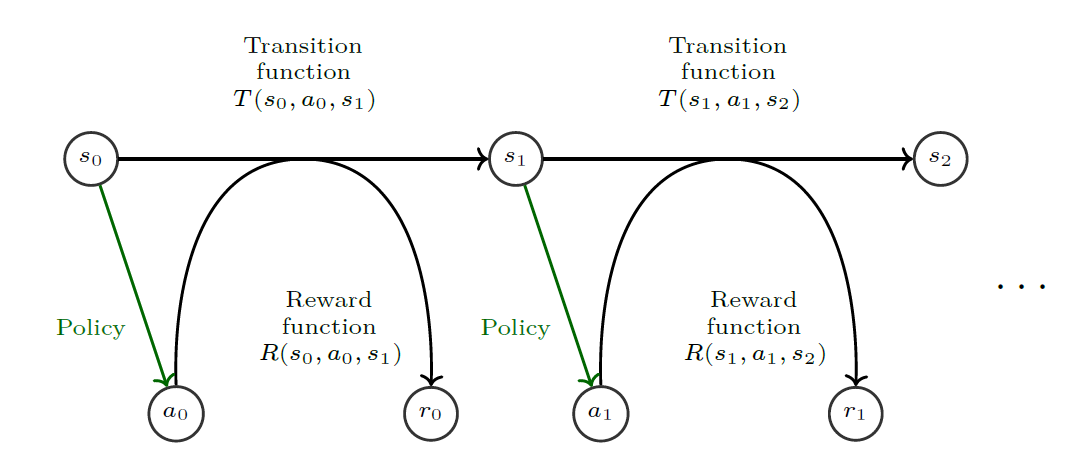
\includegraphics[width=.5\linewidth]{figs/mdp_detail.png}
\caption{Agent takes an action to move to the next state and observe a reward \protect\cite{franccois2018introduction}} \label{fig:2}
\end{figure}

One of the most popular algorithms for learning optimal policies remains Q-learning \cite{watkins1992q}. Each state in the state space has state-action pairs called Q-values. The Q-value $Q(s,a)$ describes the rewards an agent can expect from taking taking action $a$ in state $s$. For instance, if Mario encounters a Goomba in his current state, the Q-value for taking an action running into the Goomba would be lower than the Q-value for taking an action killing the Goomba. The Q-value under a policy $\pi$ is formalised as the expected sum of discounted rewards \textbf{given} state $s$ and action $a$:

\begin{equation}
 Q^\pi(s, a) = \E \left[ \sum_{k=0}^{\infty} \gamma^k R_{t+k+1} \Big| S_t = s, A_t = a \right]
\end{equation}


An optimal policy is therefore one which for each state chooses the action associated with the largest Q-value. To learn an optimal policy, an agent needs to learn the Q function: $Q : S \times A \to \R$ of the problem. Learning the Q-function is a process of continuously experiencing the environment and using the observations to update the Q-values until they converge. The following shows the Q-value update:

\begin{equation} \label{q_update}
	Q(s,a) \gets Q(s,a) + \alpha \left[ R + \gamma \max\limits_{a^\prime} Q(S^\prime, a^\prime) - Q(s,a) \right]
\end{equation}


Whenever an agent takes an action in a state and experiences a reward, the old Q-value needs to be updated to reflect that observation. This is done by adding the experienced reward $R$ for taking action $a$ in state $s$ to the discounted largest Q-value of the next state $Q(S^\prime, a^\prime)$ ($\gamma$ is the discount factor), subtracting the old Q-value, multiplying everything by the learning rate $\alpha$ and adding it to the old Q-value. The learning rate specifies the importance of new information \textit{vis-à-vis} old information. In traditional RL, the Q-function is a lookup table where each entry corresponds to a Q-value. Q-tables quickly become infeasible for complex problems however. For instance, assuming an image size of $84 \times 84$, the RGB Super Mario state space has a size of $(84 \times 84 \times 3)^{256}$. The solution is to replace the lookup table with a neural network - Deep Q Network (DQN) or policy network. This works because neural networks in essence are universal function approximators. Especially Convolutional Neural Networks (CNN) have made it possible to identify features in images and map them to outputs, thus reducing the need for a large memory footprint and allowing the application of Reinforcement Learning to high-dimensional problems like video games. A video game Deep Reinforcement Learning system usually has a \textit{policy network}. The policy network is a CNN that receives a game frame as input and outputs an action to be taken in the game. 

\begin{figure}[!htb]
\centering
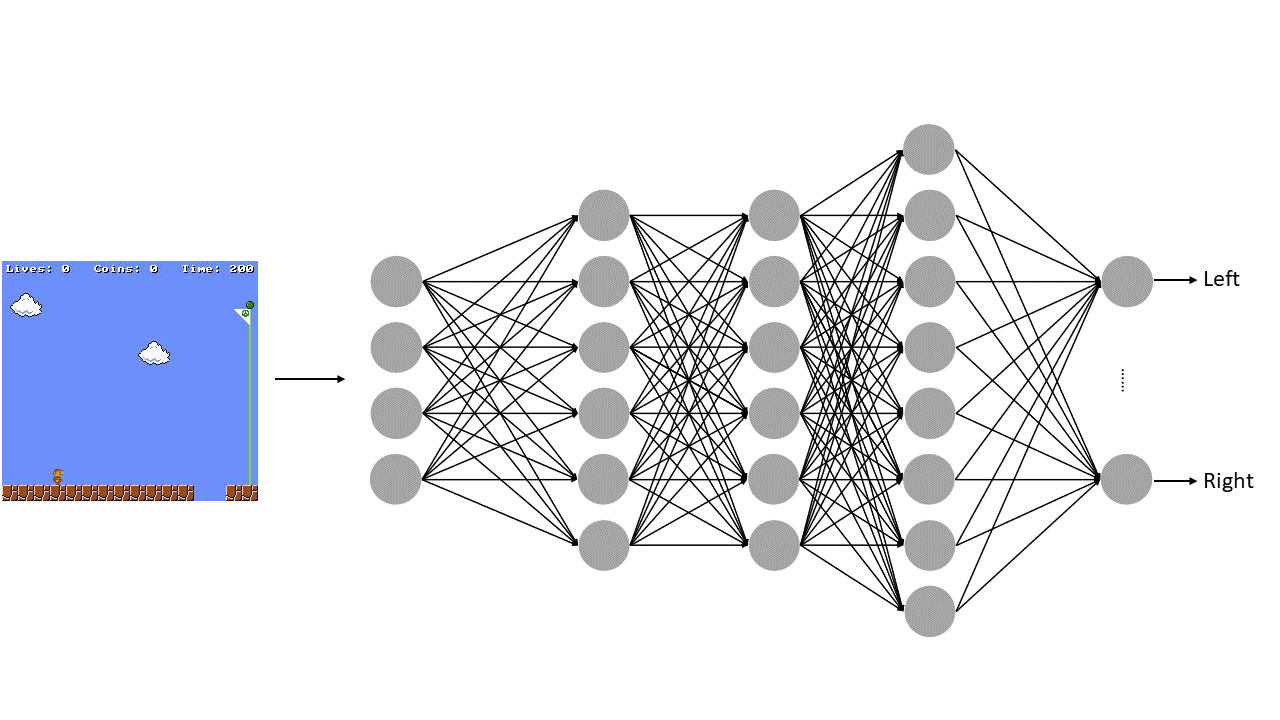
\includegraphics[trim={0 2cm 0 2cm},clip,width=1\linewidth]{figs/deep_rl_video_game.png}
\caption{Policy Network for Super Mario (not to scale)} \label{fig:2}
\end{figure}

The input first passes through a couple of convolutional layers designed to detect shapes and features such as edges and high level objects. Then follow two fully connected layers to produce the output. For Super Mario, the state is represented as a pixel matrix of dimensions $(width \times height \times channels)$ where channels is the number of colour channels in the frame - 3 for RGB, 1 for grayscale. Given a state, the CNN performs a forward pass and assigns ranks to the possible actions Mario can take, e.g. left, right, jump etc. The network has an output neuron for each possible action Mario can take in the game. Ranks in this case are the Q-values of that state and so the best action is the output neuron with the highest Q-value. Now all that remains is to train the network so that we can learn the optimal Q-values of the MDP. The principle remains the same as in the Q-update equation \ref{q_update} with the difference that the Q function is a CNN instead of a lookup-table. First, the loss of the network is calculated using a loss function, which is then differentiated with respect to the weights of the network before taking a gradient step. Ultimate goal of the learning process is for the CNN to output Q-values to approximate the optimal Q-values of the MDP. 

\subsubsection{Target Networks}
The improvement made by replacing the Q-table with a neural network is significant, however an issue arises when calculating the network loss in the Q-value update (see \ref{eq:q_update}). The loss is computed as the difference between the targeted Q-values of the next state, i.e. $Q(s^\prime, a^\prime)$, and the Q-values outputted by the network for the current state, i.e. $Q(s,a)$. Goal is for $Q(s,a)$ to approximate $Q(s^\prime, a^\prime)$, though because the policy network is used to calculate both values, any weight updates to the network will shift both $Q(s,a)$ and $Q(s^\prime, a^\prime)$. At each iteration, $Q(s,a)$ will move closer to the targeted Q-value., However the targeted $Q(s^\prime, a^\prime)$ will move as well and we end up chasing a moving target. Ultimately, this causes overestimation of the Q-values and leads to learning instabilities resulting in poor policies. The solution is to use a separate target network with the frozen weights of the policy network to calculate the target Q-values. Therefore, target Q-values remain stationary when being approximated and the network does not overestimate Q-values. Periodically, the policy network's weights are copied to the target network so that they accurately reflect the learning process.


%\begin{figure}[!htb]
%\centering
%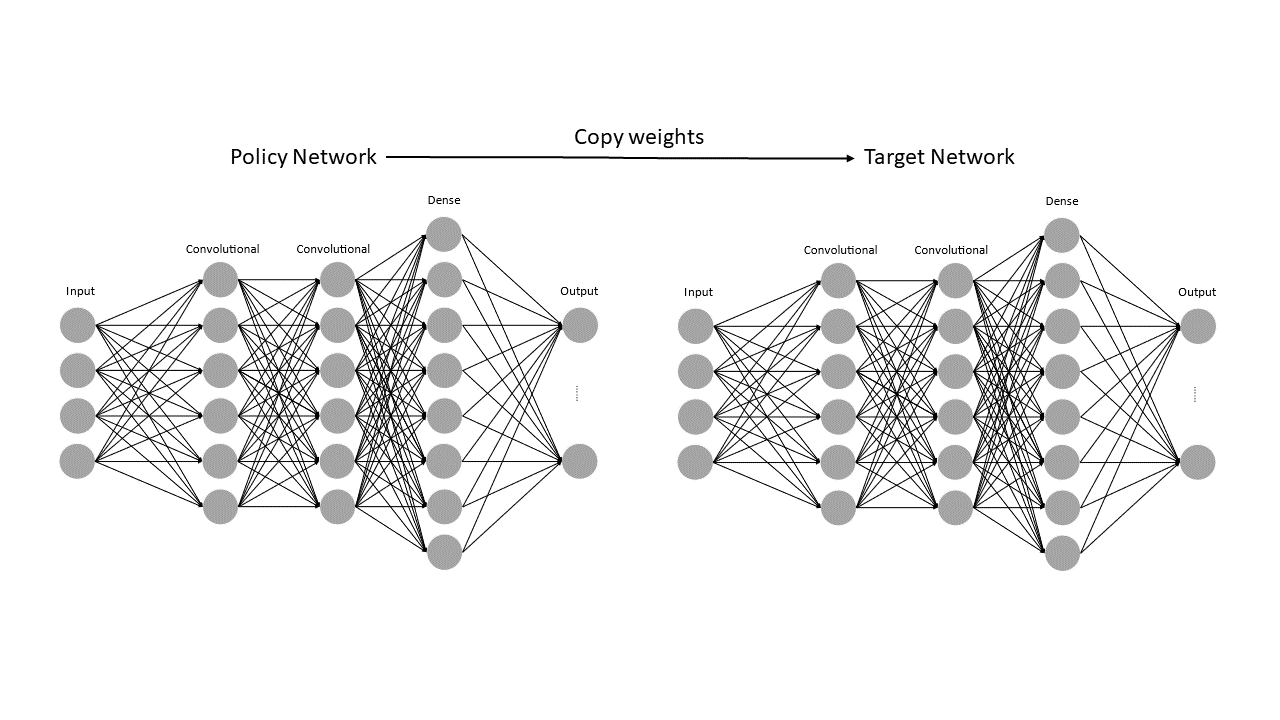
\includegraphics[trim={0 3cm 0 3cm},clip,width=1\linewidth]{figs/policy_target_nn.png}
%\caption{Policy and Target Networks} \label{fig:2}
%\end{figure}

\subsubsection{Experience Replay}
In traditional Reinforcement Learning, observations of the environment are immediately discarded after the Q-values have been updated. Experiencing the environment as a consecutive stream of temporally sequential observations becomes problematic because samples are highly correlated and training on correlated data may get you stuck in a local minimum. Furthermore, because observations are not kept, each one of them can only be used in a single weight update which makes learning less efficient. Therefore, most Deep Q Learning algorithms attempt to break correlation between samples and reuse them for weight updates with a \textit{replay memory} \cite{lin1993reinforcement}. The replay memory is a buffer of size $N$ where the agent stores experience tuples $e_t = (s_t, a_t, r_{t+1}, s_{t+1})$. Until the agent has collected a sufficient number of samples, it will execute random actions. Once the memory has been filled with enough samples, the agent randomly samples a batch and uses it to train the policy network. 


\subsection{Hierarchical Reinforcement Learning}
Arguably, one of humans' most remarkable abilities is the ability to generalise knowledge \cite{geirhos2018generalisation} across various contexts withstanding input distribution changes. For example, you are able to recognise a door as a door and open it regardless of its colour or material because you abstract away the features which make up the door and generalise it to other doors. While Deep Reinforcement Learning partially alleviates the issue of generalisation \cite{sutton1996generalization}, it remains a substantial issue \cite{van2017hybrid} to date. Reinforcement Learning agents are prone to overspecialise and overfit because they are trained and tested within the same environment \cite{cobbe2018quantifying}. If Mario is trained to solve level \textit{World 1-1}, he only becomes an expert on that particular level. When placed in the next level, he would not perform as well because Mario did not \textbf{learn} any concepts of the world. Instead, he \textbf{remembers} optimal action sequences only applicable to a distinct problem. This is also known as \textit{flat} Reinforcement Learning.

\begin{wrapfigure}{r}{0.5\textwidth}
	\vspace{-20pt}
	\begin{center}
		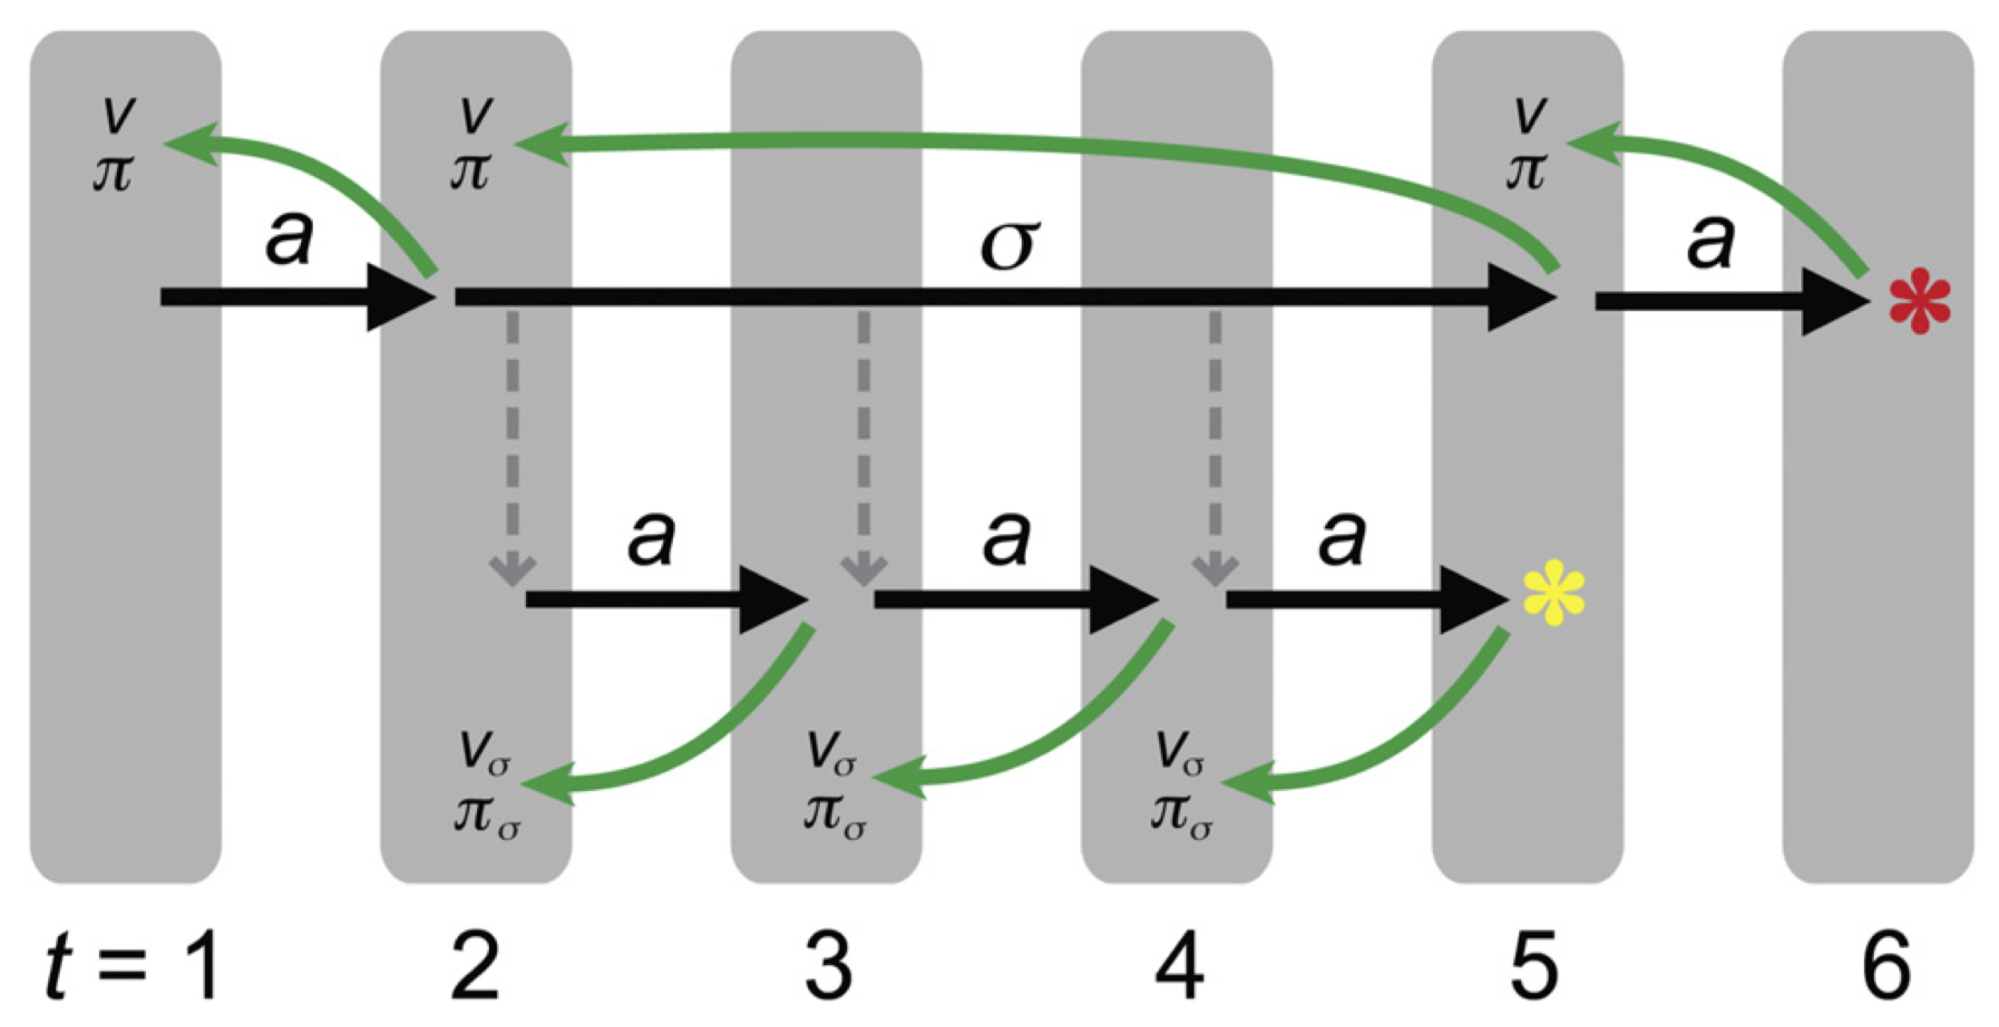
\includegraphics[width=0.4\textwidth]{figs/hrl_smdp.png}
	\end{center}
	\vspace{-20pt}
\caption{The Hierarchical RL Semi Markov Decision Process \protect\cite{ribas2011neural}} \label{fig:4}
\end{wrapfigure}

Learning reusable skills is the essence of Hierarchical Reinforcement Learning. It is inspired by the fact that human decision making is \textit{temporally abstract} \cite{sutton1999between} and hierarchically composed. When leaving work to go home, you need to exit the office, however first you need to get up from your chair and take the lift downstairs. The parent task of going home contains multiple subtasks which themselves involve subtasks of their own. By decomposing the overall problem into smaller subproblems, learning is sped up and actions can be reused across the domain. This requires some modification to the MDP used in tradiational Reinforcement Learning. Remember that in \textit{flat} learning, each action $a_t$ only lasts a single timestep. Now, the agent can execute actions lasting multiple timesteps. An action $a_t$ in state $s_t$ can transport the agent to state $s^{\prime}_{t+k}$. The policy $\pi$ is made up of multiple sub-policies, each of which are catering to a specific subset of the state space. At timestep $t_1$, the primitive action $a$ is selected and lasts one timestep. At $t_2$, the policy $\pi$ invokes a subpolicy or subtask $\sigma$ which is in charge of selecting primitive actions until $t_5$. Upon termination, the subpolicy returns a reward (yellow asterisk) back to the master policy which incorporates it into the value of the state from where the policy was invoked. What convolutional neural networks did for vision, figuring out behavioural hierarchies are to RL.

\subsubsection{Option-Critic}
The following Hierarchical algorithm is an advancement on the Markov-Options framework \cite{sutton1999between} which first introduced a framework for extending the classical one-timestep-action MDP to a multi-timestep-actions Semi MDP (SMDP). The SMDP contains \textit{Markov Options}, a layer of temporal abstraction on top of the primitive one-timestep actions of the agent. An option is defined as a triplet $\langle I, \pi, \beta \rangle$ where:

\begin{itemize}[noitemsep]
	\itemsep0em
	\item $I \subseteq S$ is the subset of states available to the option.
	\item $\pi : S \times A \to [0,1]$ is the policy for the option.
	\item $\beta : S^+ \to [0,1]$ is the termination criterion for the option.
\end{itemize}

An option can only be chosen by the agent if the current state is in the subset of states available to the option, $s_t \in I$. This restricts options to a specific portion of the state space. For every subsequent state reached in the option, it will terminate with probability $\beta(s_{t+k})$. In Sutton et. al's work, the options/subpolicies had to be handcrafted for the agent to learn and use them. Additionally, learning these subpolicies came at a great temporal and spatial expense because each option is solved as its own MDP. The Option-Critic architecture \cite{bacon2017option} improves upon this by not only discovering subpolicies autonomously, but also simultaneously learning the policy over options/master policy as well as subpolicies. The number of hierarchies is fixed at two. Furthermore, it assumes that options are available to the agent everywhere in the state space. Just like vanilla Deep Reinforcement Learning, Option-Critic utilises Deep Q Networks to approximate the Q value function.



\begin{wrapfigure}{r}{0.5\textwidth}
	\vspace{-20pt}
	\begin{center}
		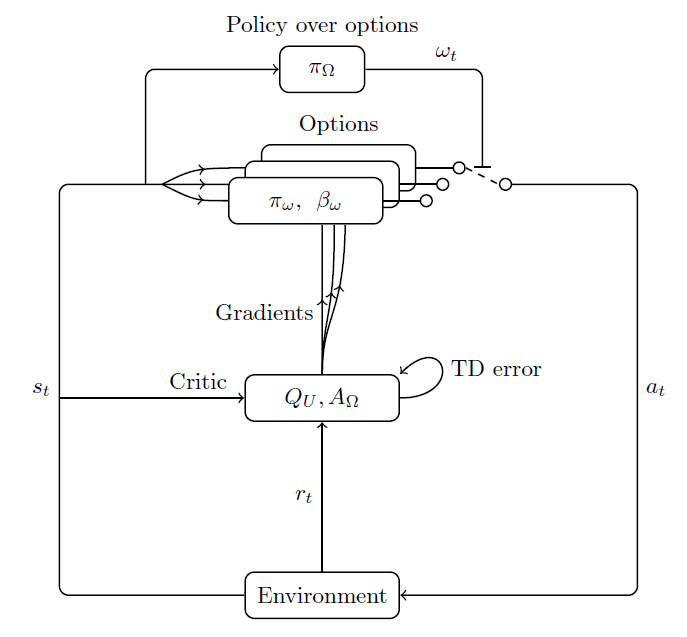
\includegraphics[width=0.4\textwidth]{figs/option_critic_architecture.png}
	\end{center}
	\vspace{-20pt}
\caption{Option-Critic Architecture \protect\cite{ribas2011neural}} \label{fig:4}
\end{wrapfigure}

At each timestep, the master policy $\pi_\Omega$ chooses an option/subpolicy $\omega_t$. We follow the regular MDP structure where the option/subpolicy executes an action $a$ in the environment and receives a reward $r$ and new state $s^\prime$ in return. The critic then evaluates the option by using the Q-value $Q_U$ of executing a subpolicy $\omega$ from state $s$ to obtain the new Q update. If the next state is a terminal state of an option, we obtain the update value $\delta$ by subtracting the observed reward $r$ from $Q_U$. Otherwise, we compute the update value like we did for a terminal state and add the discounted Q-value $Q_\Omega$ of the entire option as well as the max Q-value of the \textbf{next} option. After evaluating, the option is improved using Stochastic Gradient Descent. The option terminates when the criterion $\beta_\omega$ is fulfilled after which the policy over options/master policy chooses the next option. 

\subsubsection{Feudal Networks}
Another recent Hierarchical Reinforcement Learning algorithm is DeepMind's FeUdal Network (FuN) \cite{vezhnevets2017feudal}. Like the Option-Critic architecture, is is an improvement on an older system, called Feudal Reinforcement Learning \cite{dayan1993feudal}. Feudal Reinforcement Learning follows the general Hierarchical Reinforcement Learning architecture where different levels of temporal abstraction work together to solve the overall task. Taking after the questionable medieval feudal system, managers set goals for the sub-managers to solve in the state space and receive rewards once completed. Communication is restricted to a single hierarchical step, meaning that each level can only give goals to the sub-manager below and receive goals from the manager above. Additionally, the number of hierarchies are not fixed. Though a great improvement on standard Q-learning, traditional Feudal Reinforcement Learning is not general enough to work on multiple domains and has inherent convergence issues. DeepMind's FeUdal Network provides a fixed two-level manager-worker hierarchy encapsulating multiple neural networks. At the top is the manager, setting goals for the worker in the latent space. Working like a compass, the manager figures out \textbf{where} the worker should go. At the bottom, the worker has a high temporal resolution and is responsible for choosing primitive actions in the environment. Given a goal by the manager, the worker decides \textbf{how} to achieve it.

\begin{wrapfigure}{r}{0.5\textwidth}
	\begin{center}
		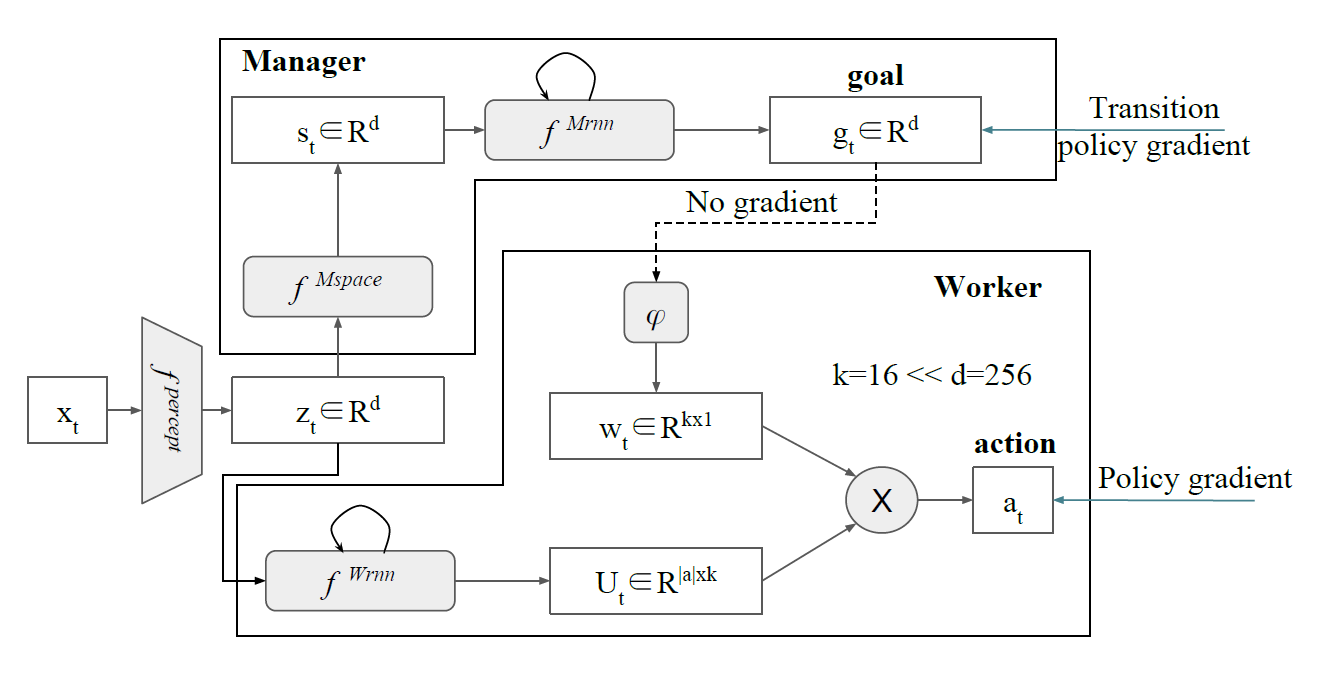
\includegraphics[width=.5\textwidth]{figs/fun_architecture.png}
	\end{center}
	\caption{FuN Architecure \protect\cite{vezhnevets2017feudal}} \label{fig:4}
\end{wrapfigure}


FuN has a more complex architecture than the regular DQN and Option-Critic systems. First, the game frame is passed through a CNN modelled after DeepMind's Atari \cite{DBLP:journals/corr/MnihKSGAWR13} network to compute a separate intermediate representation $z_t$ of the state $x_t$ to be shared between the manager and worker. After further compressing the state $z_t$ into $s_t$, the manager utilises a Long short-term memory (LSTM) Recurrent Neural Network (RNN) to compute a goal $g_t$ for the worker to solve. The worker is given the intermediate state representation $z_t$ and uses an LSTM to produce an action embedding matrix $U$ where each row corresponds to a possible action within the game. To incorporate the manager's goal, the worker then embeds it into a vector $w_t$. By applying a dot product to the action matrix $U_t$ and the goal embedding $w_t$, we get a probability distribution over the actions, making FuN a stochastic architecture. 

\section{System Requirements}

The following section specifies the requirements to be fulfilled by the system:

\begin{itemize}

	\item \textbf{Super Mario Game Emulator}\\ 
	The Reinforcement Learning agent within the system must have the ability to interact with the Super Mario Bros game environment to obtain information about states, rewards and to perform actions. The Python OpenAI Gym library provides a plugin to play Super Mario, however this plugin does not allow the creation of custom levels (more on custom levels in the next point). Instead, the sytem will use the Mario AI Tenth Anniversary Edition \cite{marioai} framework. Although written in Java, it provides the user with the ability to create their own levels using ASCII art.
	
	\item \textbf{Custom Levels}\\
	Using custom levels means that we can better investigate Mario's generalisation abilities. The agent can learn specific skills in specially designed levels and slowly expand their skillset. This is also the main reason for choosing the Mario AI Tenth Anniversary Edition framework over the OpenAI Gym library. OpenAI Gym only provides the original Super Mario levels and therefore makes the skill stacking with Hierarchical Reinforcement Learning algorithms less transparent.
	
	\item \textbf{Reward Function}\\
Every MDP has a reward function. Because the chosen Super Mario framework does not have a reward function, it will first need to be designed. The function should incentivise the intended behaviour of the agent - to move as far right as possible in the level without dying.
	
	\item \textbf{Java-Python Bridge}\\
	Because the chosen Super Mario game framework is written in Java and Python is the de facto lingua franca of Reinforcement Learning, the system needs to have a communication bridge between the languages. The system needs to train for longer periods of time, so avoiding unnecessary overhead whereever possible is important. Getting the two languages "as close" as possible to each other is therefore vital. A client-server architecture using HTTP to send JSON is easy to implement, however comes with too much overhead. The Jython \cite{jython} and JPype \cite{jpype} frameworks are directly embedded in the JVM to reduce latency, however they are not as out of the box user friendly. The Py4J \cite{py4j} framework on the other hand uses sockets to communicate with the Java API which leads to a slight performance decrease. Though it is nearly effortless to setup and easy to use which is why it is the best choice for the system.
	
	\item \textbf{Deep Learning Libraries}\\
	Contemporary Reinforcement Learning algorithms rely on Neural Networks to learn behaviour. The system needs to be able to initialise and train neural networks by making use of existing libraries. PyTorch is the most suitable option as it offers a good balance between low-level granularity and easy to use high-level API. Additionally, PyTorch has their own Reinforcement Learning tutorials.
	
	\item \textbf{Python Game Interface}\\
	The different Reinforcement Learning agents of this project all need to interact with the Super Mario Java game emulator. Writing a Python interface that bridges to the emulator and provides standard operations for the agents to use will reduce code duplication on the agents' part and decouple them from the emulator logic.
	
	\item \textbf{Preprocessing}\\
	The environment as observed by the Reinforcement Learning agent is a pixel matrix of the current frame of the game. Commonly, frames are cropped and scaled before being passed to the neural network. Cropping removes unnecessary information such as the score and timer counters at the top of the screen. Scaling reduces the complexity of the image and the number of neurons needed in the network. For to reduce latency, cropping and scaling will need to be done on the Java side of the system.
	
	\item \textbf{Monitor Training}\\
	Reinforcement Learning algorithms need to train for anything from several hours to several days. Monitoring this process while it is going on is important because bugs can be caught early on and hyperparameters are more easily compared. Tensorboard provides tools for visualising various metrics such as rewards and loss. Graphs are updated live as the training is happening and the data can be downloaded as JSON or CSV for further analysis.
	
	\item \textbf{Remote Training}\\
	The entire system needs to be able to run locally as well as remotely in the cloud. Hardware in the cloud is more powerful and can be scaled up and down as needed. Additionally, it is robust. Google Cloud provides APIs specifically designed for Machine Learning and comes with free credits for first time users. Hence it was used for training the Reinforcement Learning models.
	
\end{itemize}

	

\section{System Implementation}
The following section will describe the system architecture in detail as it was implemented from the requirements section.


\subsection{Super Mario Game}
Super Mario Bros game was released by Nintendo in 1985 and is the most iconic Super Mario game to date. It was the first Mario game to have a sidescrolling feature, i.e. where the game is viewed from the side and movement to the left or ride gradually reveals more of the level via scrolling, and introduced many of the now commonly known features such as Goombas and power ups. The goal for Mario is to get to the flag at the end of a level without dying or timing out in the process. Each level contains obstacles such as gaps, pipes, blocks and enemies like Goombas or Koopas. 


\subsection{Overall Architecture}
The system follows a client-server model where the Reinforcement Learning client uses the Py4J bridge to execute actions on the game emulator server and observe states and rewards. The client first initiates the environment via the game interface and receiving back the start state of the MDP (note that this process is not displayed in the game server diagram). Having chosen an action according to their policy, the agent passes a \textit{tensor} with said action to the game interface which encodes it as a \textit{boolean action vector}, e.g. $\begin{bmatrix} false & true & false & true & false\end{bmatrix}$ for going right. When the action vector is received by the Game Server via Py4J, the action is executed in the environment $k$ times (see section \ref{frame_stacking_skipping} for frame skipping). The final frame of the action sequence is cropped and resized (see section \ref{frame_preprocessing}) and the reward is calculated using the environment's reward function (see section \ref{reward_function}). The reward and the frame are then marshalled back to the client using Py4J and extracted by the Reinforcement Learning Agent using the game interface. At every timestep and after every completed episode, the agent writes the observed reward and the calculated loss into tensorboard. Once training has finished, the models and hyperparameters are saved for demonstration, evaluation and further training. For the 

\begin{figure}[!htb]
\centering
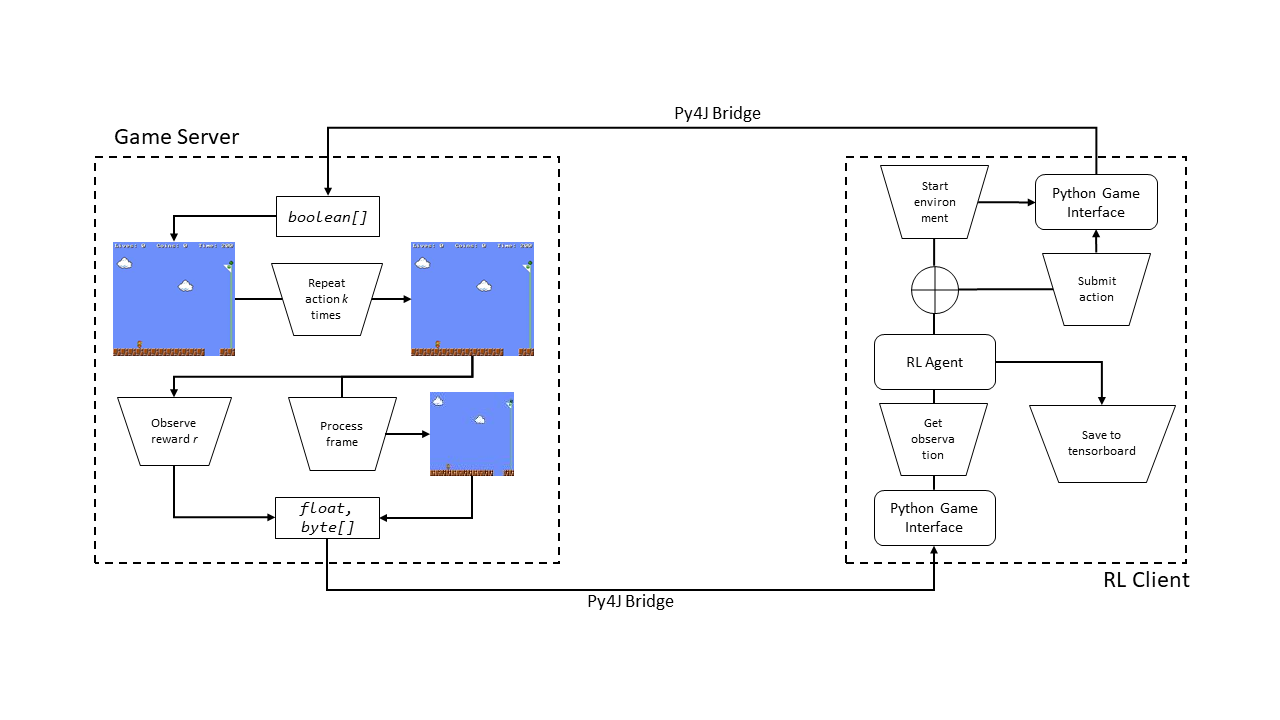
\includegraphics[trim={0 2cm 0 2cm},clip,width=1\linewidth]{figs/system_architecture.png}
\caption{System Architecture}
\end{figure}

The game server is a \textit{jar} file built using \textit{maven} exposing a port for the client to interact with. It is based on the \textit{marioai} \cite{marioai} framework which had to be partially rewritten. Various methods and classes for calculating the reward, preprocessing the game frame and exposing the observations of the environment to an outside agent. To allow for remote training, both client and server are running on a 4CPU 16GB Google Cloud virtual machine. Although only relying on CPU power to the run the system is prolonging training times, the expense of adding GPUs was considered too much for this project.


\subsection{Reward Function} \label{reward_function}

A Reinforcement Learning agent learns to distinguish between desirable and undesirable behaviour depending on the reward they illicit from the environment. At each time step $t$, the agent receives a scalar reward $R_t \in \R$ as a result of an action taken at time step $t-1$. The agents goal is to maximise the total reward it receives $\sum^{t}_{i=1} R_i$ and thus solve the task it is given. If we want to the agent to do something, it needs to receive rewards which when maximised achieve the goal we set out. It is important to note that the reward tells the agent \textit{what} it should achieve but not \textit{how} it should be achieved. Designing a reward function improperly might lead to unintended behaviour, also known as the \textit{cobra effect}. During British colonial rule in India, the government offered a reward for dead cobras as a way to reduce their population. Eventually, people began breeding cobras for income to milk the system and the program was scrapped. Breeders then set their snakes free, leading to an increase in the cobra population \cite{siebert2001kobra}. This is a pertinent example of how a flawed reward function can produce unwanted behaviour. It is important to remember that in the end, you always get the behaviour you incentivised, not always the behaviour you intended. A well-crafted reward function aligns the \textbf{incentivised} behaviour with the \textbf{intended} behaviour.

Luckily, simple video games such as Super Mario often have clear criteria for success and failure, meaning that reward function design is of relatively low complexity. We want to incentivise Mario to reach the flag at the end of the level (success) and avoid anything that results in death (failure). Giving Mario positive rewards for moving right in the level and negative rewards for moving left forces Mario to keep moving right. Additionally, providing large negative rewards in terminal failure states and large positive rewards in terminal success states further forces Mario to stay alive and move towards the flag. Positive rewards encourage the agent to keep playing and accumulating those rewards. However, an agent may potentially avoid a terminal state to keep racking up rewards. Therefore, it is important to have positive terminal state values which make the agent choose the terminal state over reward hacking. Negative rewards on the other hand encourage the agent to finish the level as quickly as possible. Besides death, the agent is also penalised each time step $t$ to avoid him standing still. Thus, the agent will want to reach a terminal state as quickly as possible. Rewards are usually bounded to avoid exploding gradients in the neural networks.
\linebreak
The reward function used in this project is inspired by the  \textit{openai gym} Super Mario Bros framework \cite{pypi}. It is composed of three variables $v, c, d$:

\begin{itemize}

	\item Velocity: $v = x_t - x_{t-1}$. The difference in the agent's \textit{x} values in between time steps $t$ and $t - 1$. Moving right will increase $v$.
	
	\item Clock: $c = c_t - c_{t-1}$. The difference in the game's clock values in between time steps $t$ and $t - 1$. For each action committed in game, $c$ will decrease by $1$. Using frame skipping \ref{frame_stacking_skipping}, each action performed by the Reinforcement Learning agent will yield a $c$ value of $-4$. This is to prevent the agent from standing still.
	
	\item Death/Win: 
		\begin{equation*}
   	 		d = \begin{cases}
               			100               & \text{Mario wins}\\
               			-100              & \text{Mario dies}\\
               			-100				 & \text{Game times out}\\
           			\end{cases}
		\end{equation*}
		
		The death and timeout penalty encourage to avoid death and finish the level as quickly as possible. The win reward is to provide an extra incentive to visit the winning terminal state. In the original game, Mario receives more points the higher up he hits the flag at the end of the level. This was not modelled in the reward function to reduce its complexity.
		
	\item The reward function $r$ is then the summation of the three variables $r(v, c, d) = v + c + d$. Additionally it is clipped in the range of $(-100, 100)$.
	
	
\end{itemize}


\subsection{Exploitation vs Exploration}\label{exploit_explore}
A major challenge within Reinforcement Learning is to strike a balance between gathering enough information about the environment (exploration) and to obtain as much reward as possible (exploitation) \cite{sutton2011reinforcement}. A greedy agent will choose the action which according to their current knowledge returns the largest reward - \textit{exploitation}. Though for an agent to exploit an action they must previously have explored it enough times to have a reliable estimate on the action's reward. Being greedy produces large short term rewards, however the agent might ignore other options with potentially even larger rewards. Performing exploration instead could uncover those options and therefore lead to more reward in the long run. The dilemma arises when at each time step, the agent must decide whether to exploit or explore the environment. Exploring too much makes the agent a slow but steady learner. Exploiting too much means that the agent will quickly converge on their choice of actions but ultimately not act optimally.

\begin{wrapfigure}{r}{0.5\textwidth}
\vspace{-40pt}
  \begin{center}
    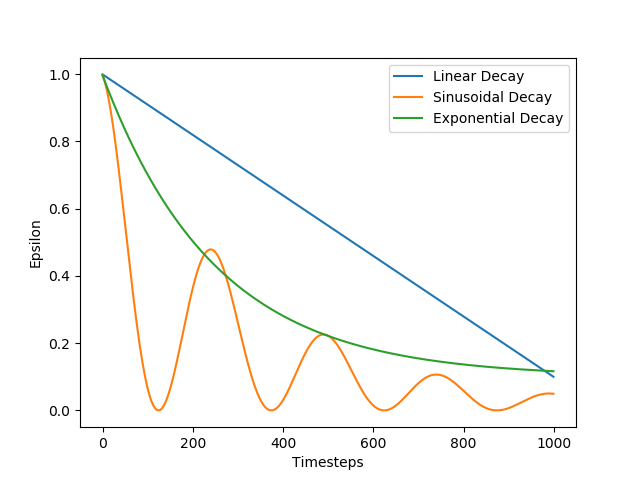
\includegraphics[width=0.48\textwidth]{figs/epsilon_decay.png}
  \end{center}
  \vspace{-20pt}
  \caption{Variants of $\epsilon$ Decay}
  %\vspace{-40pt}
\end{wrapfigure}

A popular policy for choosing between exploitation and exploration is the $\epsilon$-greedy algorithm \cite{white2012bandit}. At each timestep, the agent chooses the best action to exploit the environment with $1-\epsilon$ probability. Exploration is more desirable at the beginning of the learning process because the agent does not possess enough information about the environment yet. Hence, the value for $\epsilon$ is usually decayed over time to reflect this. Methods for decaying $\epsilon$ can be linear \cite{mnih2015human}, exponential \cite{maroti2019rbed} and sinusoidal  \cite{chuchro2017game}. The algorithms that use an $\epsilon-Greedy$ policy in this project use a linear decay.


\subsection{Frame Preprocessing} \label{frame_preprocessing}
Preprocessing data is a step all Machine Learning systems go through prior to starting the actual learning. For a Reinforcement Learning network, the input is a pixel matrix representing a game frame. For Super Mario, the dimensions of the raw image as returned by the game are $240 \times 256 \times 3$. Before the raw image can be passed to the network however, it needs to go through a series of preprocessing steps aimed at reducing its dimensionality and making learning less computationally demanding. First, unnecessary information such as the score, lives, and timer and cropped out because they do not provide relevant clues to the agent. Second, the image is resized to $84 \times 84 \times 3$ using bilinear interpolation \cite{gribbon2004novel} to further reduce the size of the neural network needed for training. The dimensions $84 \times 84$ are taken from DeepMind's \textit{Playing Atari with Reinforcement Learning} paper \cite{DBLP:journals/corr/MnihKSGAWR13}. Converting the image to grayscale is another often applied preprocessing step. Though models tend to perform lower on grayscale \cite{lample2017playing}.

\begin{figure}[!htb]
\centering
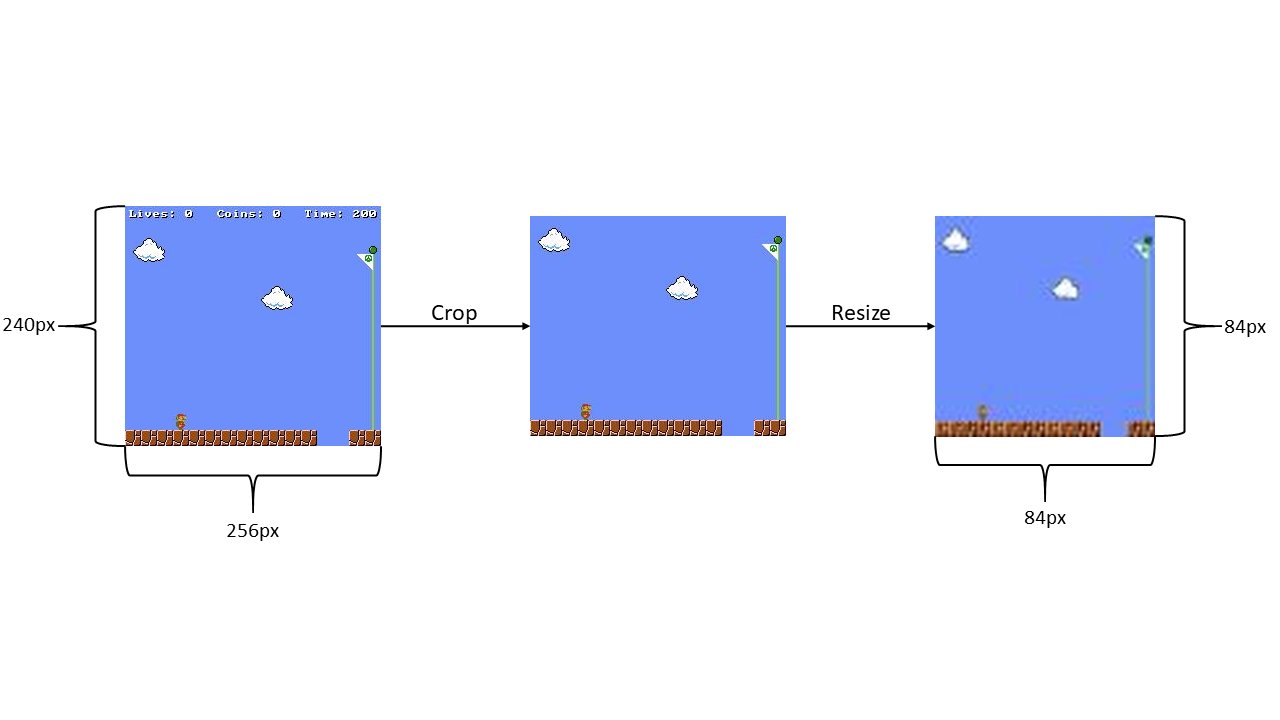
\includegraphics[trim={0 4.5cm 0 5cm},clip,width=1\linewidth]{figs/frame_preprocessing.png}
\caption{Frame Preprocessing Pipeline}
\end{figure}



\subsection{Frame Stacking and Frame Skipping} \label{frame_stacking_skipping}
When playing a video game, it is important for the player to have a sense of how the objects in the environment are moving. Looking at a single frame of Super Mario does not tell you whether Mario is moving left, right, up or down. Only when presented with consecutive frames could you actually determine Mario's movement. Hence, to give the policy network of our system an idea of where Mario is going, it is fed a stack of 4 frames as input. Using 4 frames was again pioneered by DeepMind \cite{DBLP:journals/corr/MnihKSGAWR13}.

\begin{figure}[!htb]
\centering
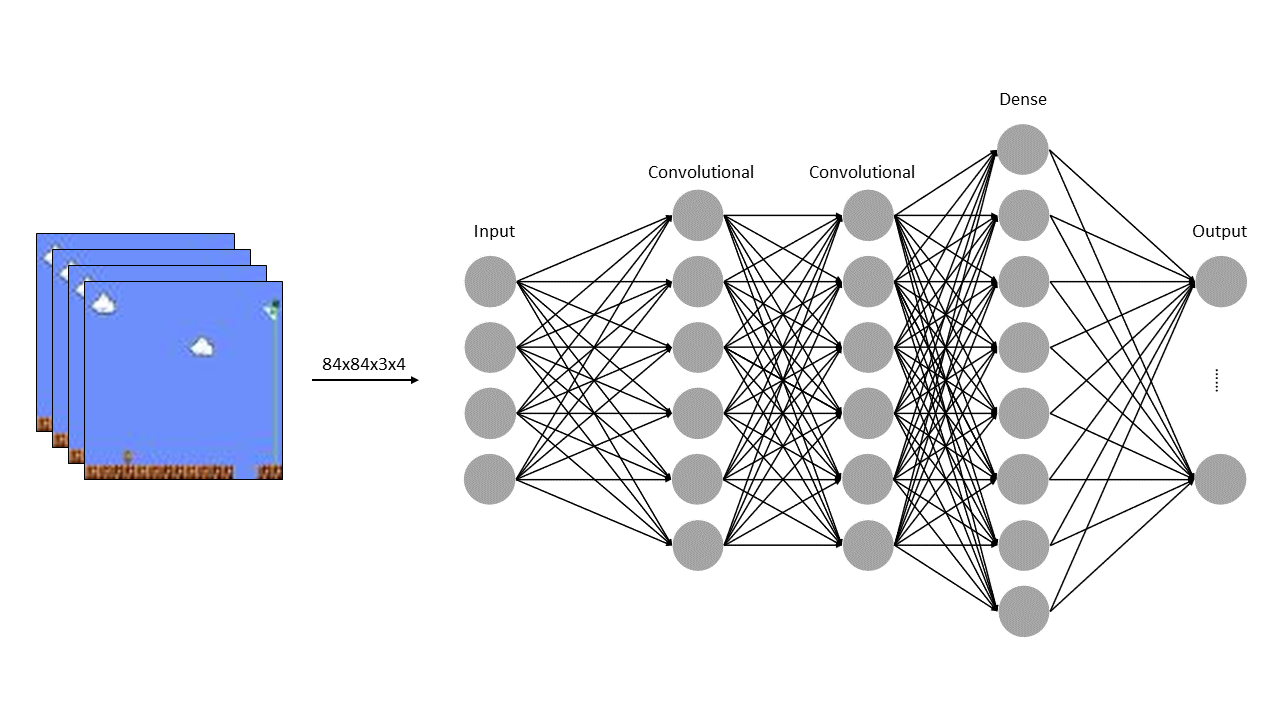
\includegraphics[trim={0 2cm 0 2cm}, clip, width=.75\linewidth]{figs/frame_stacking_nn.png}
\caption{Stacked frames are given as input to the neural network. The dimension of the input thus becomes $84 \times 84 \times 3 \times 4$}.
\end{figure}

Another trick DeepMind used in their paper is to only show the agent every $k^{th}$ frame of the game. Instead of taking an action for every frame in the game, the agent now decides on an action every $k^{th}$ frame. The chosen action is then repeated for $k-1$ frames. This idea is partially motivated by how humans would play the game. A human player makes decisions on how to proceed in the game not for every frame they observe, but at intervals depending on the game environment (some games require faster reactions than others). Using frame-skipping also has the benefit of speedier learning because executing actions in the emulator is faster than making the agent choose an action. Choosing a value for $k$, one must factor in the desired resolution granularity. A large value for $k$ means that episodes can be played faster, however the agent might miss out on opportunities in the game because the same action is repeated too many times \cite{braylan2015frame}. On the other hand, agents may learn associations between temporally distant states and actions when skipping a large amount of frames. A small $k$ gives the agent finer granularity, though at the cost of longer episodes. 


%\begin{figure}[!htb]
%\minipage[t]{0.48\textwidth}
%  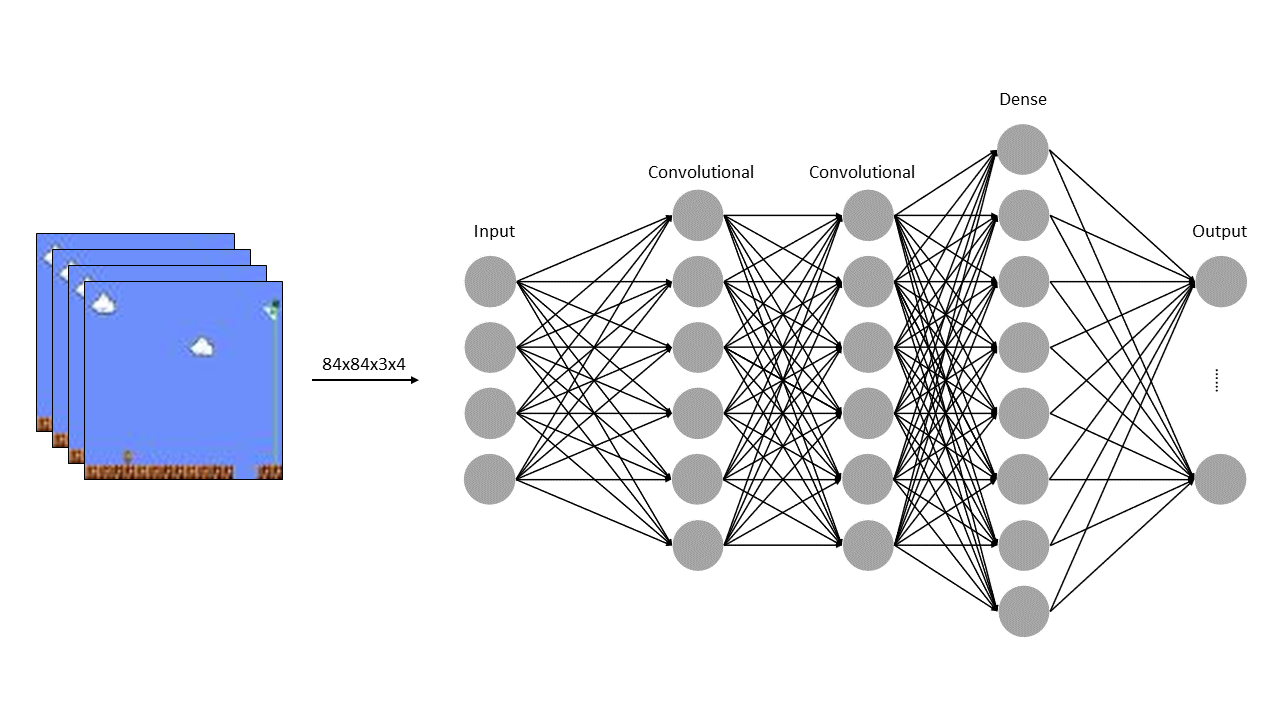
\includegraphics[trim={0 2cm 0 2cm}, clip, width=\linewidth]{figs/frame_stacking_nn.png}
%  \caption{Stacked frames are given as input to the neural network. The dimension of the input thus becomes $84 \times 84 \times 3 \times 4$}\label{fig:steps_gap_level}
%\endminipage\hfill
%\minipage[t]{0.48\textwidth}
%  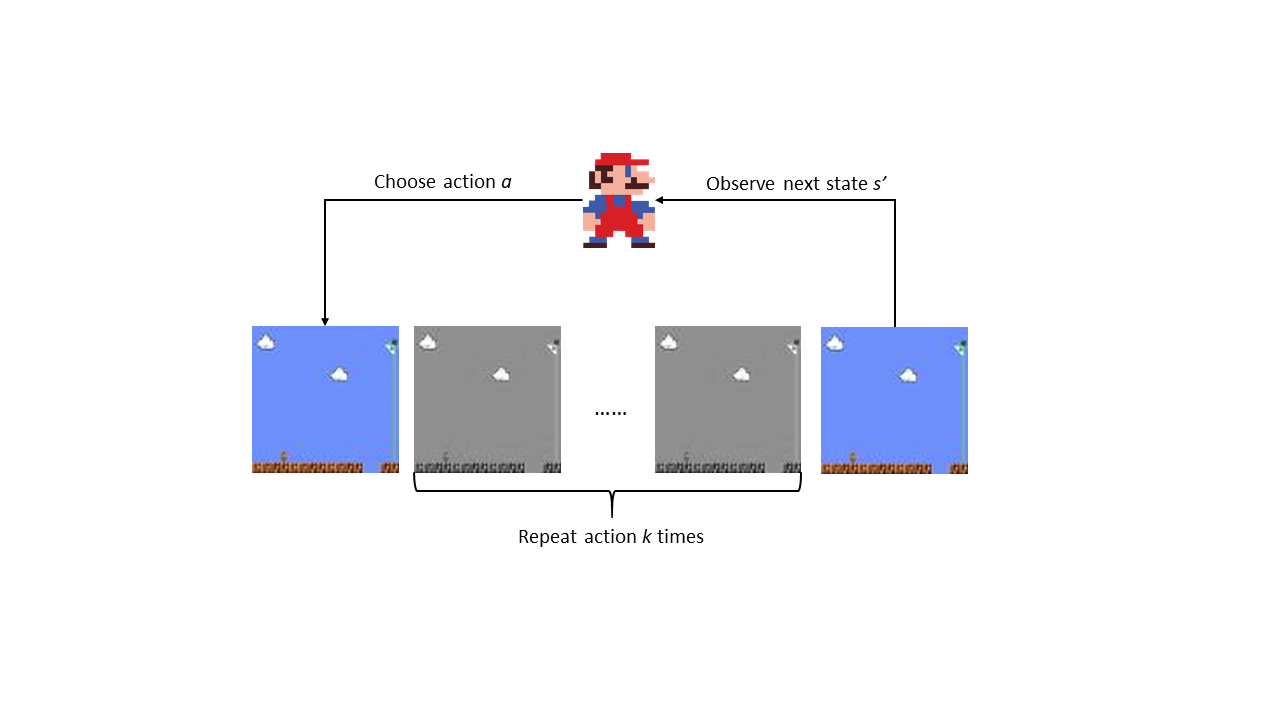
\includegraphics[trim={0 4cm 0 4cm}, clip, width=\linewidth]{figs/frame_skipping.png}
%  \caption{The agent selects action $a$ to be executed $k$ times in the emulator and observes the $k^{th}$ frame}\label{fig:}
%\endminipage\hfill
%\end{figure}


\begin{figure}[!htb]
\centering
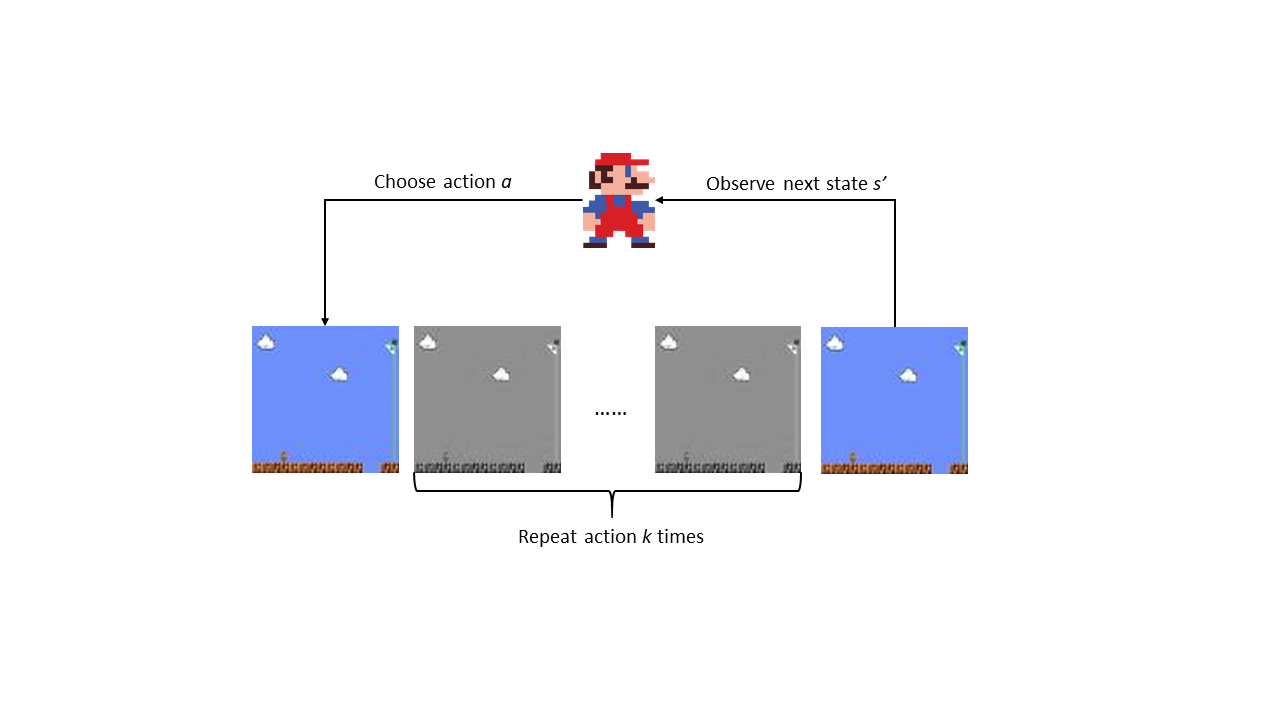
\includegraphics[trim={0 4cm 0 4cm}, clip, width=1\linewidth]{figs/frame_skipping.png}
\caption{The agent selects action $a$ to be executed $k$ times in the emulator and observes the $k^{th}$ frame}.
\end{figure}

\subsection{Custom Levels}\label{custom_levels}
Investigating whether agents can learn skills and reuse is best done with custom levels. A custom level represents a skill the agent ought to learn and therefore provides a closed off space where learning can take place. The project used three custom built levels - two where agents were meant to learn a basic skill, as well as a third one which is a combination of the two basic levels. Regardless of the skill that agents are supposed to learn, the goal is still to reach the flag at the end. In the system, levels are \texttt{.txt} file with ASCII art and can rapidly be created and changed if needed. The three levels created for this project were:

\begin{enumerate}
	\item \textbf{Steps with Gap}\\
	In this level, the skill to be learned is to jump up the steps and across the gap to reach the flag on the other side.
	
	
	\item \textbf{Two Pipes}\\
	In this level, the agent needs to learn how to jump over pipes. Though it also involves jumping, overcoming a pipe requires a different set of primitive actions than crossing steps with a gap.
	
	\item \textbf{Steps with Gap + Two Pipes}\\
	A combination of the previous two levels, the agent needs to overcome pipes as well as steps with a gap in the middle before reaching the flag.
\end{enumerate}


	\begin{figure}[!htb]
\minipage[t]{0.25\textwidth}
  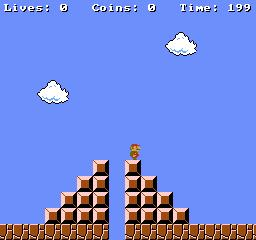
\includegraphics[width=\linewidth]{figs/steps_gap_level.png}
  \caption{Steps with Gap Level}\label{fig:steps_gap_level}
\endminipage\hfill
\minipage[t]{0.25\textwidth}
  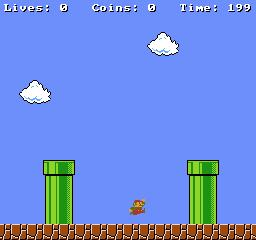
\includegraphics[width=\linewidth]{figs/two_pipe_level.png}
  \caption{Two Pipes Level}\label{fig:}
\endminipage\hfill
\minipage[t]{0.25\textwidth}%
  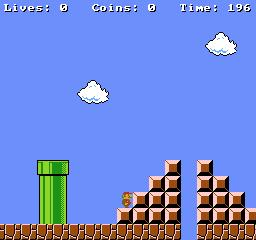
\includegraphics[width=\linewidth]{figs/steps_pipe_level.png}
  \caption{Steps with Gap + Two Pipes}\label{fig:awesome_image3}
\endminipage
\end{figure}

The project is confined to only teaching Mario navigation tasks, hence why none of the levels include any enemies. The reasoning behind this is the state space associated with dynamic and static objects. Pipes, gaps, and steps are static objects that do not move around in the world. A Goomba or Koopa on the other hand is dynamic and forces Mario to learn more states before knowing how to act around it.



\section{Experiment Design}
The goal of this project is to investigate whether introducing hierarchies and temporal abstraction into Reinforcement Learning speeds up the learning process. A good indicator of a model's learning process is how quickly it is able to accumulate rewards. Models that learn quickly, will have discovered actions which return large rewards sooner than slow learning models. Therefore, the main metric used to compare the different Reinforcement Learning models will be the average reward per episode. To judge whether learning hierarchies is beneficial to learning speed, the same Mario model is trained sequentially on three levels. The first two levels are designed for Mario learn specific skills - navigating steps and jumping over pipes respectively (section \ref{custom_levels}). The third level is a combination of the two previous levels and requires the previously learned skills to be solved. An agent which has learned reusable hierarchies should in theory adopt to the new environment faster than a flat-learning agent. Adopting in this sense means to acquire rewards faster. In addition to comparing the different learning agents against each other in the new environment, the agents will also be compared against versions of themselves which have not been trained on previous levels. The purpose of this comparison is to investigate whether training agents \textit{sequentially} is beneficial over learning from scratch.

Determining the stopping criterion, i.e. when the model should stop learning, was grounds to some experimentation. Using the number of episodes played the agent is common, however episodes vary in length across different levels as well as in the same level. This variation means that agents will have had different amount of playtime as better agents would finish sooner and there is no guarantee that agents get the same experience. The goal was to let all agents experience the same number of frames of the game to better predict training times and to use the number of episodes as a metric of success instead. A fast-learning agent should be able to play through more episodes using the same number of timesteps than a slow-learning agent. Thus, the completed number of episodes after $t$ timesteps can also be used to compare the different Reinforcement Learning models. To summarise, an agent which learns quickly should achieve more rewards in fewer episodes.

\begin{table}[h!]
\centering
\begin{tabular}{ |c|c|c|c|c|c| } 
 \hline
 \textbf{Model} & \textbf{Level} & \textbf{sequential} & \textbf{Frames} & \textbf{Runtime}\\
 \hline 
 DQN & Steps with Gap & False & $2 \times 10^5$ & 1d 3h 54m 59s\\ 
 \hline
 DQN & Two Pipes & False & $2 \times 10^5$ & 1d 5h 31m 54s\\ 
 \hline
 DQN & Steps with Gap + Two Pipes & False & $2 \times 10^5$ & 1d 5h 46m 34s \\ 
 \hline
DQN & Two Pipes & True & $2 \times 10^5$ & 1d 6h 58m 31s\\ 
 \hline
 DQN & Steps with Gap + Two Pipes & True & $2 \times 10^5$ & 1d 5h 59m 9s\\ 
 \hline 
 Option Critic & Steps with Gap & False & $2 \times 10^5$ & 1d 8h 33m 34s\\ 
 \hline
 Option Critic & Two Pipes & False & $2 \times 10^5$ & 1d 17h 35m 37s\\ 
 \hline
 Option Critic & Steps with Gap + Two Pipes & False & $2 \times 10^5$ & 1d 9h 32m 13s\\ 
 \hline
Option Critic & Two Pipes & True & $2 \times 10^5$ & 1d 19h 33m 13s\\ 
 \hline
 Option Critic & Steps with Gap + Two Pipes & True & $2 \times 10^5$ & 1d 13h 7m 29s\\ 
 \hline
 
  FuN & Steps with Gap & False & $2 \times 10^5$ & 1d 14h 40m 8s\\ 
 \hline
 FuN & Two Pipes & False & $2 \times 10^5$ & 1d 13h 58m 52s\\ 
 \hline
 FuN & Steps with Gap + Two Pipes & False & $2 \times 10^5$ & 1d 12h 13m 18s\\ 
 \hline
FuN & Two Pipes & True & $2 \times 10^5$ & 1d 17h 14m 25s\\ 
 \hline
 FuN & Steps with Gap + Two Pipes & True & $2 \times 10^5$ & 1d 14h 4m 24s\\ 
 \hline
 
\end{tabular}
\caption{Experiments carried out for the project. sequential indicates whether the model has been pretrained on another level already.}
\label{tbl:experiments}
\end{table}

All experiments were run once on a Google Cloud 4CPU 15GB RAM virtual machine. While it is desirable to run experiments multiple times to ensure that the observations do not represent noise, financial limitations and long training times only allowed a single run per experiment. 

\section{Results}

\subsection{DQN Agent}\label{dqn_experiment}
Using a DQN as a comparison baseline is common in the Reinforcement Learning literature \cite{bacon2017option, kulkarni2016hierarchical, hessel2018rainbow, levy2017learning}, thus this project will follow the trend. This section will show how the Deep Reinforcement Learning theory from section \ref{deep_rl} was used to construct a DQN agent and compare the average reward per episode for sequential and non-sequential models. The DQN agent uses a policy and target network, both of which are CNNs with three convolutional layers followed by two linear layers. The activation function used between the layers is a Rectified Linear Unit (ReLu) \cite{lecun2015deep}, which over the past years established itself as the most popular activation function for training neural networks \cite{ramachandran2017searching}. The agent also makes use of experience replay with a buffer of size 100,000. 

\begin{figure}[!htb]
\vspace{-40pt}
\centering
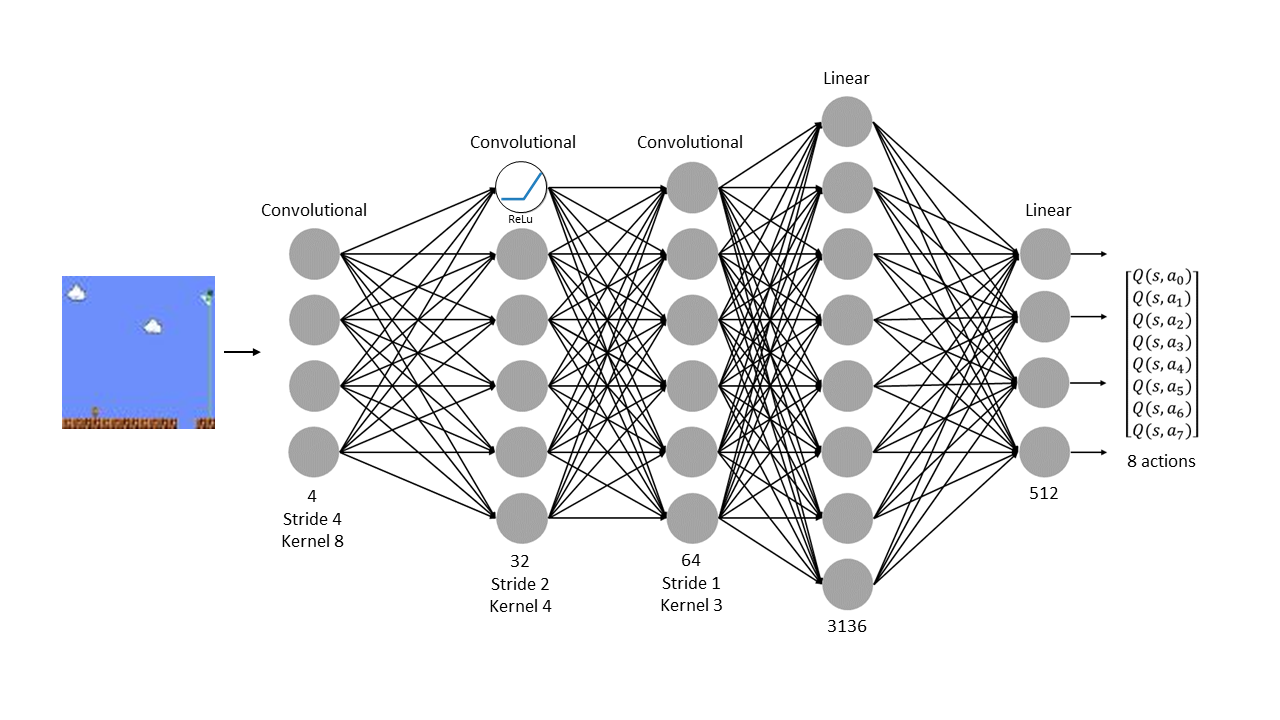
\includegraphics[trim={0 0 0 0}, clip, width=1\linewidth]{figs/dqn.png}
\vspace{-20pt}
\caption{Illustration of the CNN used by the DQN Agent (not to scale). Stride is the number of pixels the convolutional filter moves. Kernel is the size of the filter.}
\label{fig:dqn_cnn}
\end{figure}

Choosing the hyperparameters for a model is an important aspect. Performing a grid search \ref{bergstra2012random} for optimising parameters would have been to costly considering the time it takes to run each experiment. Therefore, parameters values commonly appearing in the Reinforcement Learning literature and various implementations of the DQN algorithm were chosen.

\begin{table}
	\begin{tabular}{ |c|c|c|c|c|c|c|}
	\hline
	\textbf{$\alpha$} & \textbf{Batch Size} & \textbf{$\gamma$} & \textbf{Buffer Size} & \textbf{Target Update Freq} & \textbf{Learn Freq} & \textbf{Learn Start}\\
	\hline
	0.0001 & 32 & 0.99 & 100,000 & 200 & 4 & 50,000 \\
	\hline
	\end{tabular}
	\captionsetup{singlelinecheck=off}
	\caption[DQN Hyperparameters]{DQN Hyperparameters where: \begin{itemize}
	\itemsep0em 
		\item \textbf{$\alpha$}: Learning Rate.
		\item \textbf{Batch Size}: The number of samples used to train the network each training epoch.
		\item \textbf{$\gamma$}: Discount Factor.
		\item \textbf{Buffer Size}: Size of the replay buffer.
		\item \textbf{Target Update Freq}: Frequency in timesteps the weights from the policy net are copied to the target net.
		\item \textbf{Learn Freq}: Frequency in timesteps the network is trained, e.g. every 4th frame.
		\item \textbf{Learn Start}: When the agent should start sampling from the replay memory and train the network.
	\end{itemize}}
	\label{tbl:dqn_hyperparams}
\end{table}


\begin{figure}[t]
     \centering
     \begin{subfigure}[t]{0.32\textwidth}
         \centering
         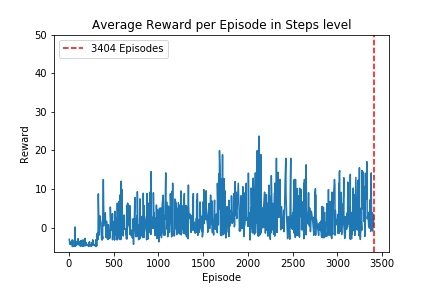
\includegraphics[width=\textwidth]{figs/dqn_results_1.png}
         \caption{}
         \label{fig:dqn_results_1}
     \end{subfigure}
     \hfill
     \begin{subfigure}[t]{0.32\textwidth}
         \centering
         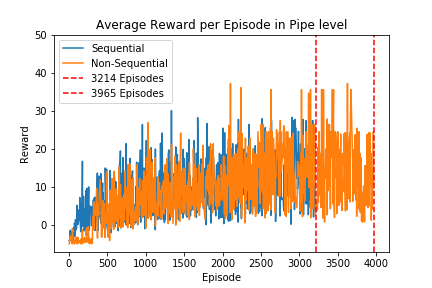
\includegraphics[width=\textwidth]{figs/dqn_results_2.png}
         \caption{}
         \label{fig:dqn_results_2}
     \end{subfigure}
     \hfill
     \begin{subfigure}[t]{0.32\textwidth}
         \centering
         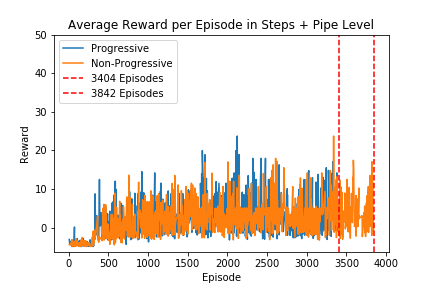
\includegraphics[width=\textwidth]{figs/dqn_results_3.png}
         \caption{}
         \label{fig:dqn_results_3}
     \end{subfigure}
        \caption{DQN Performance on the three Super Mario levels measured in the average reward per played episode.}
        \label{fig:dqn_results}
\end{figure}

\begin{table}[h!]
\centering
\begin{tabular}{ |c|c|c|c|c|c| } 
	\hline
	\textbf{Levels} & Steps & sequential Pipe & Pipe & Steps + Pipe & sequential Steps + Pipe\\
	\hline
	\textbf{Final Rewards} & 242.34 & 225.76 & 322.24 & -25.0 & 242.34 \\
	\hline
	\textbf{Total Rewards} & 388.12 & 2485.56 & 4483.92 & -228.09 & 388.12 \\
	\hline
\end{tabular}
\caption{Rewards accumulated by the DQN agent in each level. Final rewards are the total rewards acquired in the final episode of the run. Total rewards is the sum of all rewards of the run.}
\end{table}

The DQN agent was able to mostly find successful policies for all three levels, accumulating mostly positive rewards in all except the Steps + Pipe level when trained from scratch. A successful policy should lead to a net positive reward for the agent in the very last episode of the run. In the last episode, the agent is fully exploiting the environment by only choosing optimal actions. Hence, if the agent has learned a successful policy it is expected that the total reward in the last episode is positive. The results also show that a sequential agent who has been trained on the steps level is able to accumulate rewards faster at first in the pipe level when compared to an agent who has to learn the level from scratch (see the first 250 episodes in \ref{fig:dqn_results_2}). Thereafter, the two models have nearly identical reward curves however. The non-sequential agent manages to accumulate a higher reward in the final episode of the run, suggesting that the model learned a better policy. Looking at the total rewards per run, it can be confirmed that the non-sequential model accumulated more in total as well. In the final level where the steps and pipes were combined to test Mario's abilities to reuse information (\ref{fig:dqn_results_3}), both the sequential and non-sequential model learned at about equal speeds. Although here the sequential model appears to have found a more successful policy as it has more rewards in the final episode as well as over the entire run.


\subsection{Option-Critic Agent}\label{oc_experiment}
The Option Critic implementation follows that of a DQN with the addition of the options framework on top. It is an added layer of complexity, which shows in the experiment runtimes - learning the additional subpolicies takes extra time. Option Critic uses a CNN with the same structure as the DQN (see \ref{fig:dqn_cnn}) to learn policies and utilises a policy and target network to avoid overestimating Q-values. Additionally, it also uses the concept of experience replay with a replay buffer of size 100,000 to store observation tuples in and utilises the DQN values for the rest of the hyperparameters as well (see \ref{tbl:dqn_hyperparams}). Lastly, the number of options to be learned was specified at 2, taking after the authors of the Option Critic paper \cite{bacon2017option}. The code was sourced from public github repositories \cite{oc_github} and adapted to fit the specifications of the project.


\begin{figure}[htb!]
     \centering
     \begin{subfigure}[t]{0.32\textwidth}
         \centering
         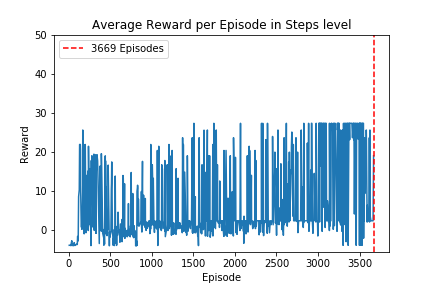
\includegraphics[width=\textwidth]{figs/oc_results_1.png}
         \caption{}
         \label{fig:oc_results_1}
     \end{subfigure}
     \hfill
     \begin{subfigure}[t]{0.32\textwidth}
         \centering
         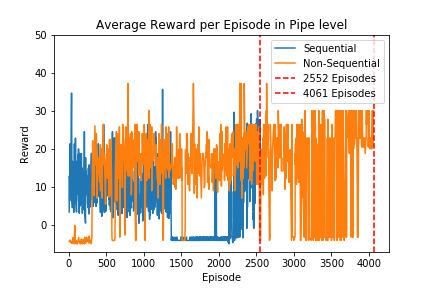
\includegraphics[width=\textwidth]{figs/oc_results_2.png}
         \caption{}
         \label{fig:oc_results_2}
     \end{subfigure}
     \hfill
     \begin{subfigure}[t]{0.32\textwidth}
         \centering
         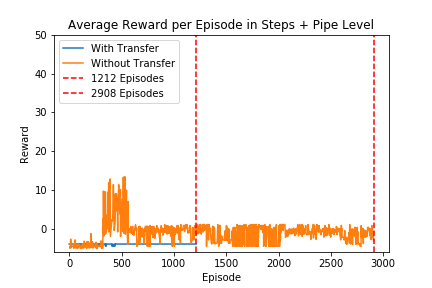
\includegraphics[width=\textwidth]{figs/oc_results_3.png}
         \caption{}
         \label{fig:oc_results_3}
     \end{subfigure}
        \caption{Option Critic Performance on the three Super Mario levels measured in the average reward per played episode.}
        \label{fig:oc_results}
\end{figure}

\begin{table}[htb!]
\centering
\begin{tabular}{ |c|c|c|c|c|c| } 
	\hline
	\textbf{Levels} & Steps & sequential Pipe  & Pipe & Steps + Pipe & sequential Steps + Pipe \\
	\hline
	\textbf{Final Rewards} & 342.47 & 336.71 & 420.62 & -309.0 & -629.0\\
	\hline
	\textbf{Total Rewards} & -471.95 & 186.54 & 4492.79 &  -2687.05 & -3870.95 \\
	\hline
\end{tabular}
\caption{The total sum of credits accumulated in each level by the Option Critic agent.}
\label{tbl:oc_rewards}
\end{table}

Overall, the performance of the Option Critic is very erratic and unstable in all levels. The average reward obtained per episode goes through extreme fluctuations from values just below zero up to values of thirty. As the episode count goes up the agent is meant to slowly converge on a master policy which returns more rewards than a policy earlier in the run. Though Option Critic agent appears to only be showing minimal improvement over the duration of a run, its final policies actually outperform the DQN on the Steps, sequential Pipe, and Pipe runs (see Final Rewards in Table \ref{tbl:oc_rewards}). Like the DQN, the results show that a sequential agent who has been trained on a previous level is to quicker to adapt to the new environment (see the first 250 episodes in \ref{fig:oc_results_2}). Adapting quickly means to require fewer episodes to finding actions which return larger rewards. However, the non-sequential model outperforms the sequential model in the late stages of the run for both the Pipe and Steps + Pipe levels (see final and total rewards in Table \ref{tbl:oc_rewards}). Occasionally, the Option Critic gets stuck in local minima which can be seen as the flat sections with low reward values in the reward curve (see sequential \ref{fig:oc_results_2} and sequential \ref{fig:oc_results_3}). It indicates that Mario has gotten stuck somewhere in the level and keeps accumulating the negative reward for letting the time pass. The agent manages to leave the local minimum in the Pipe level but not in the Steps + Pipe level.


%Why OC failed?
%* not enough options
%* only tested on a simple domains

\subsection{FuN Agent}\label{fun_experiment}
The implementation of the FuN agent differs from that of the DQN and Option Critic. Though it also has a CNN with ReLu activation functions, the number of layers as well as values for stride and kernel are different. This is because the CNN does not compute the Q-values but an intermediate state representation that is to be used further down the processing pipeline. Because FuN uses recurrent networks in the form of LSTMs to compute an action distribution for the agent, the architecture can do without the concept of memory replay and target networks. Hence, FuN has a lower memory footprint than both the DQN and Option Critic which might have to store millions of experiences for more complex problems. The intricate design of the FuN agent is more computationally expensive however as can be seen in the experiment runtimes (see Table \ref{tbl:experiments}). As with the Option Critic and DQN agent, the code for the FuN agent was taken from a public github repository \cite{fun_github} and altered to fit the project specifications.

\begin{figure}[htb!]
     \centering
     \begin{subfigure}[t]{0.32\textwidth}
         \centering
         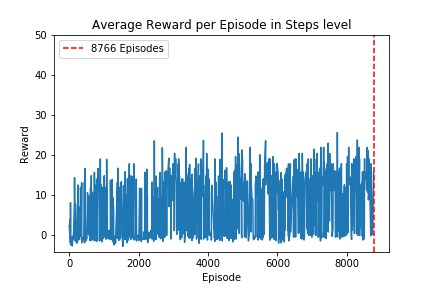
\includegraphics[width=\textwidth]{figs/fun_results_1.png}
         \caption{}
         \label{fig:fun_results_1}
     \end{subfigure}
     \hfill
     \begin{subfigure}[t]{0.32\textwidth}
         \centering
         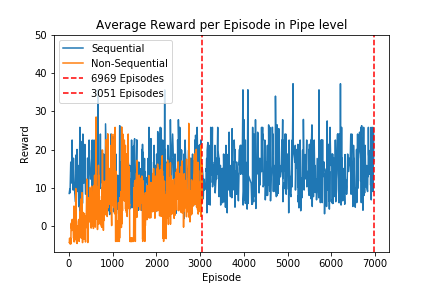
\includegraphics[width=\textwidth]{figs/fun_results_2.png}
         \caption{}
         \label{fig:fun_results_2}
     \end{subfigure}
     \hfill
     \begin{subfigure}[t]{0.32\textwidth}
         \centering
         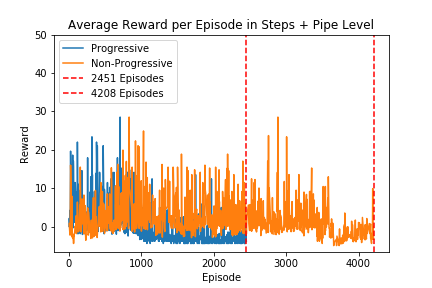
\includegraphics[width=\textwidth]{figs/fun_results_3.png}
         \caption{}
         \label{fig:fun_results_3}
     \end{subfigure}
        \caption{FuN Performance on the three Super Mario levels measured in the average reward per played episode.}
        \label{fig:fun_results}
        
\end{figure}

\begin{table}[htb!]
\centering
\begin{tabular}{ |c|c|c|c|c|c| } 
	\hline
	\textbf{Levels} & Steps & sequential Pipe  & Pipe & Steps + Pipe & sequential Steps + Pipe \\
	\hline
	\textbf{Final Reward} & 330.47 & 408.62 & 283.04 & -409.73 & -629.0 \\
	\hline
	\textbf{Total Rewards} & 6595.49 & 11032.36 & 2166.36 & 694.201 & -2541.22 \\
	\hline
\end{tabular}
\caption{The total sum of credits accumulated in each level by the FuN agent.}


\end{table}

Out of the three agents, the FuN agent was able to accumulate the most total rewards in the Steps, sequential Pipe and Steps + Pipe level. It also outperformed the DQN on the final rewards in the Steps and the sequential Pipe level. As with the DQN and Option Critic, the sequential model which was trained on the Steps level outperforms that of a model which learns the level from scratch (see the first 1000 episodes in \ref{fig:fun_results_2}). Whereas the sequential DQN and Option Critic models were outperformed by the non-sequential counterparts later in the run, the sequential FuN does better than the non-sequential FuN in the final reward and total reward. Much like the the Option Critic, FuN has a worse performance than the DQN on the final Steps + Pipe level. 

\subsection{Evaluation of Results}
Comparing the sequential models against non-sequential models showed that sequential models have an initial advantage over non-sequential models when being placed in a new environment. They accumulate rewards quicker in the beginning because the weights of the policy network have already been trained on a somewhat related environment. Thus, the models becomes equipped with previous knowledge they can use to their favour. The next step is to compare how the various sequential models perform when being placed in a novel environment. A flat learning agent like the DQN should accumulate knowledge of lower quality than the the hierarchical agents because it does not have temporally abstract actions available. Quality of knowledge in this case is measured by its reusability. Knowledge which can be transferred to new spaces is highly reusable and of high quality. Likewise, knowledge which is only applicable to a narrow space is of poor reusability and thus low quality. The Option Critic and FuN agent are expected to learn reusable subpolicies which should translate to higher quality knowledge and therefore more rewards in the novel environment. 

\begin{figure}[htb!]
     \centering
     \begin{subfigure}[t]{0.48\textwidth}
         \centering
         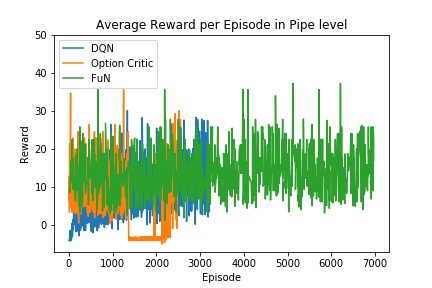
\includegraphics[width=\textwidth]{figs/all_results_1.png}
         \caption{}
         \label{fig:all_results_1}
     \end{subfigure}
     \hfill
     \begin{subfigure}[t]{0.48\textwidth}
         \centering
         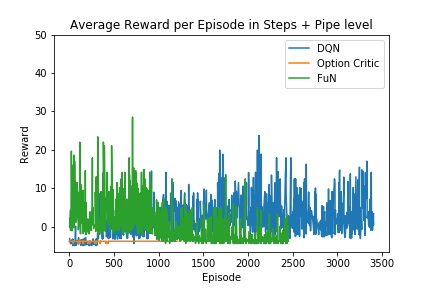
\includegraphics[width=\textwidth]{figs/all_results_2.png}
         \caption{}
         \label{fig:fun_results_2}
     \end{subfigure}
     \hfill
        \caption{Comparing the average rewards per episode for the two levels where models were pretrained.}
        \label{fig:all_results}
       
\end{figure}

Comparing the average rewards per episode for all three sequentially trained algorithms shows that the hierarchical models have an initial advantage over the DQN in the Pipe level. Both the FuN and Option Critic agent are able to obtain higher rewards than the DQN in the first 1,000 episodes of the run. This suggests that they learned reusable hierarchies in the Steps level they were previously trained on. Additionally, the learned hierarchies are superior to the learning achievements of the DQN because they allowed the agents to choose actions which lead to higher rewards. Though the DQN catches up with the hierarchical models later, initially it cannot capitalise on the information from the previous Steps level as much as hierarchical models. The same cannot be said for the the final Steps + Pipe level however as it gives inconclusive results on whether hierarchical models can exploit previously learned knowledge. The FuN agent initially obtains high rewards but converges to a suboptimal policy. The Option Critic is stuck in a suboptimal policy from the start and the DQN starts out with low rewards but is able to find a successful policy in the end. There may be reason to think that training already trained models on new environments causes them to forget what they previously learned. This would explain the inconsistent results for the performance of sequential models compared against non-sequential models for the average rewards per episode for the Steps + Pipe level in the previous sections (\ref{dqn_experiment}, \ref{oc_experiment}, \ref{fun_experiment}). Whereas the sequential FuN model learned quicker than its counterpart, the opposite was true for the Option Critic whereas the DQNs learned at around the same speed. Therefore, it can only be concluded that hierarchical sequential models have an initial learning advantage going from the Steps to the Pipe level. Adding another level to the sequence appears to cause something known as \textit{catastrophic forgetting}. When neural networks are continuously learning new tasks, the weights that were used to solve task A are overwritten to meet the objective of task B \cite{kirkpatrick2017overcoming}. When the network is given task A after learning task B, it has "forgotten" how to solve it. Having learned how to navigate steps and pipes in the first two levels, the various agents fail to reuse that knowledge in the final level which combines the two, because the network weights have been overwritten.

\subsection{Further Policy Analysis}
\begin{wrapfigure}{r}{0.5\textwidth}
\vspace{-40pt}
  \begin{center}
    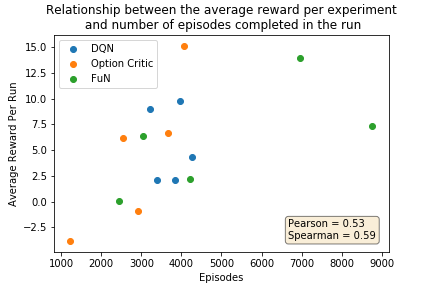
\includegraphics[width=0.48\textwidth]{figs/good_policy.png}
  \end{center}
  \vspace{-20pt}
  \caption{The average reward per run and the number of completed episodes. Pearson is a linear correlation coefficient. Spearman is a nonlinear correlation coefficient.}
  \label{fig:good_policy}
  %\vspace{-40pt}
\end{wrapfigure}

Sequentially trained hierarchical agents are faster learners when being shown a new environment (atleast for a task sequence of length 2), but are they able to find better policies? An agent can have a fast learning speed but in the end only find suboptimal policies. It was postulated that an agent who is a fast learner will achieve more rewards faster and play more episodes in the same amount of frames. Using the number of completed episodes shows that the non sequential models were able to play more episodes with the exception of the sequential FuN on the pipe level and the sequential DQN on the steps + pipe level. However, only relying on the number of completed episodes is not a reliable indicator of a good policy. Playing more episodes does not necessarily correlate with finding a better policy, it just means that you are able to finish an episode faster. An agent acting according to a policy which forces them to commit suicide immediately is able to play many episodes, but will accumulate low rewards. Therefore, looking at the number of completed episodes as the only variable variable will give the illusion of a good policy. Only where the number of completed episodes correlates positively with an overall higher reward can it be concluded that the policy is superior. Figure \ref{fig:good_policy} shows a moderate positive correlation between the number of episodes completed by an agent and the averaged average reward per episode per run. Broadly speaking, the higher the number of episodes completed, the higher the average reward. Thus, an agent that plays more episodes generally ends up with a good policy too. Although, it cannot be concluded that the hierarchical models were able to find better policies than the DQN as figure \ref{fig:good_policy} shows no discernible pattern for the different algorithms.  

\section{Deviations From Original Specifications}
The project mostly adhered to the original specifications written down at the beginning with two exceptions. First, communication between the RL agents and game emulator was supposed to happen with JSON using HTTP requests. After trialling this method it was deemed to slow and exchanged for the faster Py4J bridge. Second, the set of hierarchical algorithms to be tested included the original Options framework and an approach called Multiplicative Compositional Policies (MCP). The Options framework was substituted for the Option Critic model which is a more recent extension of it and was therefore deemed more reflective of the contemporary Reinforcement Learning literature. The MCP was exchanged for DeepMind's Feudal Network because of the lack of information and code available, both of which spoke in DeepMind's favour instead.


\section{Critical Assessment of Project}
This section will assess various of the project to see whether any changes or expansions could have benefited the project. Moreover, there are additional components which if added could have positively contributed to the project. 

\begin{itemize}
	\item
	\textbf{Experiment Runtimes}\\
	A big problem with the project was the long runtime of the experiments. The cumulative and average runtime of all experiments was 22 days, 44 minutes, 20 seconds and 1 day, 11 hours, 14 minutes and 57 seconds respectively. As a consequence, each experiment could only be run once which means that very little data could be collected. Averaging the results of multiple runs would have given a more definitive representation of the effect that sequential learning and hierarchical algorithms have on the various agents' learning abilities. With a single run per experiment however, the collected data is less reliable unfortunately. More experiments could potentially have given answers to questions like why the DQN outperforms the Option Critic and FuN on the Steps + Pipe level or why the Option Critic tends to get stuck in local optima. Additionally, the excessively long runtimes prevented discovering good values for hyperparameters which would have required further experiments. There are a number of reasons why experiments ran slow, some of which are outlined below.
	
	
	
	\item
	\textbf{Emulator Development}\\
	The Java framework used for the emulator did not meet the project requirements right out of the box. It was missing endpoints for the Python agents, classes for extracting the frames from the game as well as preprocessing, and methods for playing the game in a step by step manner. Although necessary for the success of the project, developing all of these functionalities took away valuable time from running experiments because finishing the emulator was a prerequisite for being able to run the entire system.
	
	\item
	\textbf{Slow Game Emulator Speed}\\
	Choosing the less popular \textit{marioai} Java version over the Python \textit{openaigym} version as a game emulator allowed for the easy creation of custom levels, however came at the cost of decreased emulator speed. First, the communication overhead from the Py4J bridge slowed down the agents because they had to wait for a response to be marshalled back to them. Second, the Java emulator had a ceiling for the maximum number of frames per second (fps). Thus, even with more powerful hardware the agents were constrained to a set speed and learning was slowed down.
	
	%\item
	%\textbf{Short Experiments}\\
%	As a consequence of the slow emulator speed, each experiment only ran for 200,000 frames of the game. Reinforcement Learning's sample inefficiency however requires many more frames to be effective. 
	
	\item
	\textbf{Additional Levels}\\
	The experiments showed that sequential hierarchical models are quicker to adopt to a new environments than non-sequential traditional models. To further solidify this notion it would be desirable to train the agents in different levels. This would be to make sure that the difference in performance is not due to the level environment but the agents themselves.
	
	\item	
	\textbf{Exploration Function}\\
	All agents used a linear function to calculate the exploration value $\epsilon$ (see section \ref{exploit_explore}). In multiple experiments, the Option Critic got stuck in local optima. While it is difficult to pin down the exact reason, trialing a non-linear exploration function such as the sinusoidal function \cite{chuchro2017game} which continously moves between more exploration to more exploitation over the course of an experiment could have produced different results. 
	
	\item
	\textbf{Metric for MDP Distance}\\
	An important thing to know when transferring knowledge from one environment to the next is how closely related they are. Figuring out the difference between the two environments makes it possible to assess the learning abilities in a more scientific manner. Using environments which are too similar might lead to an effect where agents perform well in the second environment because of chance and not because they learned something in the first one. Metrics such as the Hausdorff or Kantorovich metric which can be used to measure the distance between MDPs \cite{song2016measuring} could have been implemented to determine the difference between levels in Super Mario and construct levels of varying degree.
	
	\item
	\textbf{Egocentric Learning} \\
	The allocentric state representation for the MDP as an $84 \times 84$ RGB image could have been substituted for a lower-dimensional egocentric view of the game. In allocentric learning, the agent sees the entire environment (screen) whereas an egocentric agent only sees Mario's immediate surroundings. Using an egocentric view of the environment, Mario will only take into account the objects that are close to him when learning \cite{byrne2008principle}. This means that many more of the states in the state space are similar and will therefore invoke a similar response from the agent. The state space reduction means fewer states for the agent to learn and therefore a reduced experiment runtime.
	
	\item
	\textbf{Visualise Options}\\
	An interesting addition which would have helped with the analysis of the various algorithms is the visualisation of the hierarchies learned by the agents. The FuN and Option Critic agents both learned temporally abstract behaviour in the various levels, however just looking at the average reward episode does not tell when and where the agent used that behaviour. Additionally, just because the agent learned hierarchies does not mean that these hierarchies are useful. Therefore, showing which hierarchies the agents learned could have been useful in explaining the obtained results.
	
	
\end{itemize}


\section{Conclusion}

\pagebreak

\bibliographystyle{ieeetran}
\bibliography{references}

Abbeel, P. and Schulman, J. (2015). CS 294: Deep Reinforcement Learning, Fall 2015. UC Berkely.\\\\
Arulkumaran, K., Deisenroth, M., Brundage, M. and Bharath, A. (2017). Deep Reinforcement Learning: A Brief Survey. IEEE Signal Processing Magazine, 34(6), pp.26-38.\\\\
Bellman, R. E. (1957). Dynamic Programming. Princeton University Press, Princeton.\\\\
%Bellemare, M., Naddaf, Y., Veness, J. and Bowling, M. (2013). The Arcade Learning Environment: An Evaluation Platform for General Agents. Journal of Artificial Intelligence Research, 47, pp.253-279.\\\\
Bellemare, M. G., Dabney,W., and Munos, R. (2017). A distributional perspective on reinforcement learning. In the International Conference on Machine Learning (ICML).\\\\
Botvinick, M., Niv, Y. and Barto, A. (2008). Hierarchically organized behavior and its neural foundations: A reinforcement learning perspective. Cognition, 113(3), pp.262-280.\\\\
Borges, D. (2018). The Curse of Dimensionality!. [online] Medium. Available at: https://medium.com/diogo-menezes-borges/give-me-the-antidote-for-the-curse-of-dimensionality-b14bce4bf4d2 [Accessed 15 Nov. 2019].\\\\
Bradtke, S.J. and Duff, M.O. (1995). Reinforcement learning methods for continuous-time Markov decision problems, in: Advances in Neural Information Processing Systems 7, MIT Press, Cambridge, MA, pp. 393–400.\\\\
Cobbe, K., Klimov, O., Hesse, C., Kim, T. and Schulman, J. (2019). Quantifying Generalization in Reinforcement Learning. In: Proceedings of the 36 th International Conference on Machine Learning (ICML).\\\\
Dawes, G. (2017). Ancient and Medieval Empiricism (Stanford Encyclopedia of Philosophy/Winter 2017 Edition). [online] Plato.stanford.edu. Available at: https://plato.stanford.edu/archives/win2017/entries/empiricism-ancient-medieval/ [Accessed 14 Nov. 2019].\\\\
%Dayan, P. and G. E. Hinton. (1993). Feudal reinforcement
learning. In: Advances in Neural Information Processing
Systems 5, Morgan Kaufmann, San Mateo, CA, pp. 271–278.\\\\
Deepmind. (2019). AlphaStar: Mastering the Real-Time Strategy Game StarCraft II. [online] Available at: https://deepmind.com/blog/article/alphastar-mastering-real-time-strategy-game-starcraft-ii [Accessed 18 Nov. 2019].\\\\
Diuk, C., Cohen, A. and Littman, M. (2008). An object-oriented representation for efficient reinforcement learning. Proceedings of the 25th international conference on Machine learning - ICML '08.\\\\
Fler-Berliac, Y. (2019). The Promise of Hierarchical Reinforcement Learning. [online] The Gradient. Available at: https://thegradient.pub/the-promise-of-hierarchical-reinforcement-learning/ [Accessed 18 Nov. 2019].\\\\
Geirhos, R., Temme, C., Rauber, J., Schütt, H., Bethge, M. and Wichmann, F. (2018). Generalisation in humans and deep neural networks. In: Neural Information Processing Systems (NIPS).\\\\
Guestrin, C., Koller, D., Gearhart, C., \& Kanodia, N. (2003). Generalizing plans to new environments in relational mdps. IJCAI. pp. 1003–1010.\\\\
Hessel, M., Modayil, J., van Hasselt, H., Schaul, T., Ostrovski, G., Dabney, W., Horgan, D., Piot, B., Azar, M., and Silver, D. (2018). Rainbow: Combining Improvements in Deep Reinforcement Learning. In the Thirty-Second AAAI Conference on Artificial Intelligence (AAAI).\\\\
Justesen, N., Bontrager, P., Togelius, J. and Risi, S. (2019). Deep Learning for Video Game Playing. IEEE Transactions on Games, pp.1-1.\\\\
Keramati, R., Whang, J., Cho, P. and Brunskill, E. (2018). Strategic Exploration in Object-Oriented Reinforcement Learning. Published at the Exploration in Reinforcement Learning Workshop
at the 35th International Conference on Machine Learning,
Stockholm, Sweden.\\\\
Konidaris, G., Kaelbling, L. and Lozano-Perez, T. (2018). From Skills to Symbols: Learning Symbolic Representations for Abstract High-Level Planning. Journal of Artificial Intelligence Research, 61, pp.215-289.\\\\
%Kulkarni, T. D., Narasimhan, K., Saeedi, A., and Tenenbaum, J. (2016) Hierarchical deep reinforcement learning: Integrating temporal abstraction and intrinsic motivation. In Advances in neural information processing systems, 2016, pp. 3675–3683.\\\\
Minsky, M. (1961). Steps towards Artificial Intelligence. Proceedings of the IRE, 49(1), pp.8-30.\\\\
Mnih, V., Kavukcuoglu, K., Silver, D., Graves, A., Antonoglou, I., Wierstra, D., and Riedmiller, M. (2013). Playing atari with deep reinforcement learning. In NIPS Deep Learning Workshop.\\\\
%Yan, Q., Liu, Q., \& Hu, D. (2010). A hierarchical reinforcement learning algorithm based on heuristic reward function. In Advanced Computer Control (ICACC), 2010 2nd International Conference on (Vol. 3, pp. 371-376). IEEE. \\\\
Peng, X., Chang, M., Zhang, G., Abbeel, P. and Levine, S. (2019). MCP: Learning Composable Hierarchical Control with Multiplicative Compositional Policies. NeurIPS.\\\\
Posner, M. I., \& Cohen, Y. (1984). Components of Visual Orienting. In H. Bouma, \& D. Bowhuis (Eds.), Attention and Performance X (pp. 531-556). Hillsdale, NJ: Erlbaum.\\\\
Puterman, M. (2005). Markov Decision Processes: Discrete Stochastic Dynamic Programming. Hoboken, New Jersey: John Wiley \& Sons.\\\\
Scholz, J., Levihn, M., Isbell, C. L., and Wingate, D. (2014).
A Physics-Based Model Prior for Object-Oriented MDPs.
In Proceedings of the 31st International Conference on Machine Learning (ICML).\\\\
Seijen, H., Fatemi, M., Romoff, J., Laroche, R., Barnes, T. and Tsang, J. (2017). Hybrid Reward Architecture for Reinforcement Learning. In: 31st Conference on Neural Information Processing Systems (NIPS 2017).\\\\
Stolle, M., and Precup, D. (2002). Learning options in reinforcement learning. In Abstraction, Reformulation and Approximation, 5th International Symposium, SARA Proceedings, 212–223.\\\\
Sutton, R. (1995). Generalization in Reinforcement Learning: Successful Examples Using Sparse Coarse Coding. In: Neural Information Processing Systems (NIPS).\\\\
Sutton, R. and Barto, A. (2014). Reinforcement Learning: An Introduction. 2nd ed. Cambridge, Massachusetts: The MIT Press.\\\\
Sutton, R., Precup, D. and Singh, S. (1999). Between MDPs and semi-MDPs: A framework for temporal abstraction in reinforcement learning. Artificial Intelligence, 112(1-2), pp.181-211.\\\\
Vezhnevets, A. S., Osindero, S., Schaul, T., Heess, N., Jaderberg, M., Silver, D., and Kavukcuoglu, K. (2017). Feudal networks for hierarchical reinforcement learning. Proceedings of the 34th International Conference on Machine Learning - Volume 70. Pages 3540-3549.\\\\

\end{document}